\documentclass[10pt,letterpaper]{article}
\usepackage[margin=0.80in]{geometry}
\usepackage[T1]{fontenc}
\usepackage[utf8]{inputenc}
\usepackage{microtype}
\usepackage{amsmath,amssymb,mathtools}
\usepackage{graphicx,booktabs,tabularx,array,longtable,float}
\usepackage[table]{xcolor}
\usepackage{enumitem,caption,titlesec,fancyhdr,placeins,needspace}
\usepackage[numbers,sort&compress]{natbib}
\usepackage{tikz,listings}
\usetikzlibrary{arrows.meta,positioning}
\usepackage{xurl}
\usepackage[colorlinks=true,linkcolor=black,citecolor=black,urlcolor=black,breaklinks=true]{hyperref}
\newif\ifanonymous
\anonymousfalse
\newcommand{\PaperTitle}{Learning from Earlier Actions: Layered Memory for ARC-AGI-3 Agents}
% The same title as it is set on the first page, with the line break after the colon.
\newcommand{\PaperTitleBlock}{Learning from Earlier Actions:\\Layered Memory for ARC-AGI-3 Agents}
\newcommand{\PaperShortTitle}{Claude Opus 5.5 on ARC-AGI-3}
\newcommand{\AuthorName}{Chongwei (Alan) Dai}
\newcommand{\AuthorBlock}{%
  Chongwei (Alan) Dai\\[3pt]
  {\footnotesize\href{mailto:alandai06@outlook.com}{\texttt{alandai06@outlook.com}}}\\[5pt]
  {\small University of California, Los Angeles}
}
% Sole author, as confirmed by Chongwei Dai on November 23, 2026.
\newcommand{\PaperDate}{November 25, 2026}
\newcommand{\ModelName}{Claude Opus 5.5}

\definecolor{ink}{HTML}{000000}
\definecolor{accent}{HTML}{235C83}
\definecolor{muted}{HTML}{000000}
\definecolor{wash}{HTML}{F1F5F8}
\newcolumntype{Y}{>{\raggedright\arraybackslash}X}
\newcolumntype{P}[1]{>{\raggedright\arraybackslash}p{#1}}
\newcommand{\code}[1]{\nolinkurl{#1}}
% One board from the evaluated runs, with a thin frame: \board[width]{file in figures/runs}
\newcommand{\board}[2][0.30\linewidth]{{\setlength{\fboxsep}{0pt}\setlength{\fboxrule}{0.3pt}\fcolorbox{black!50}{white}{\includegraphics[width=#1]{figures/runs/#2}}}}
\newlength{\zoomw}% width of one small board in the worked example (Figure of Section 3.3.1)
% A board with labels drawn on it: \begin{markedboard}[width]{file} TikZ commands \end{markedboard}.
% Inside, (0,0) is the board's bottom-left corner and (1,1) its top-right; a cell is 1/64 wide.
\newenvironment{markedboard}[2][0.30\linewidth]{\begin{tikzpicture}[note/.style={font=\scriptsize,fill=white,fill opacity=0.88,text opacity=1,inner sep=1.5pt,align=left},pointer/.style={-{Stealth[length=1.6mm]},line width=0.6pt}]\node[anchor=south west,inner sep=0pt] (img) at (0,0) {\includegraphics[width=#1]{figures/runs/#2}};\draw[black!50,line width=0.3pt] (img.south west) rectangle (img.north east);\begin{scope}[x={(img.south east)},y={(img.north west)}]}{\end{scope}\end{tikzpicture}}
\setlength{\parindent}{0pt}
\setlength{\parskip}{3pt}
\setlength{\emergencystretch}{2em}
\setlength{\tabcolsep}{5pt}
\renewcommand{\arraystretch}{1.13}
\setlist[itemize]{leftmargin=1.3em,itemsep=2pt,topsep=3pt}
\setlist[enumerate]{leftmargin=1.6em,itemsep=2pt,topsep=3pt}
\captionsetup{font=small,labelfont=bf,skip=5pt}
\titleformat{\section}{\large\bfseries\color{ink}}{\thesection}{0.65em}{}
\titleformat{\subsection}{\normalsize\bfseries\color{ink}}{\thesubsection}{0.65em}{}
\titleformat{\subsubsection}{\normalsize\bfseries\color{ink}}{\thesubsubsection}{0.65em}{}
\titlespacing*{\section}{0pt}{9pt}{4pt}
\titlespacing*{\subsection}{0pt}{7pt}{3pt}
\titlespacing*{\subsubsection}{0pt}{5pt}{3pt}
\pagestyle{fancy}\fancyhf{}
\fancyhead[L]{\small\color{muted}\PaperShortTitle}
\fancyhead[R]{\small\color{muted}Research paper}
\fancyfoot[C]{\small\thepage}
\setlength{\headheight}{14pt}
\renewcommand{\headrulewidth}{0.3pt}
\hypersetup{pdftitle={\PaperTitle},pdfsubject={Layered evidence and memory on 25 public ARC-AGI-3 games, with confirmed final replay and full 25-game resource accounting},pdfauthor={\AuthorName}}
\lstset{basicstyle=\ttfamily\footnotesize,breaklines=true,breakatwhitespace=false,columns=fullflexible,keepspaces=true,showstringspaces=false,frame=single,rulecolor=\color{accent!30},backgroundcolor=\color{wash},aboveskip=6pt,belowskip=7pt,xleftmargin=3pt,xrightmargin=3pt}
\title{\PaperTitleBlock}
\makeatletter
\renewcommand{\@maketitle}{%
  \newpage\null\vskip-0.5em
  \begin{center}
    {\LARGE\bfseries\@title\par}\vskip0.9em
    {\normalsize\@author\par}\vskip0.7em
    {\small\@date\par}
  \end{center}\vskip0.6em
}
\makeatother
\author{\AuthorBlock}
\date{\small \PaperDate}
\setlength{\textfloatsep}{10pt plus 2pt minus 2pt}
\setlength{\floatsep}{10pt plus 2pt minus 2pt}
\setlength{\intextsep}{9pt plus 2pt minus 2pt}
% Let a large figure share its page with text; on a page of figures only, start at the top.
\renewcommand{\topfraction}{0.92}
\renewcommand{\bottomfraction}{0.75}
\renewcommand{\textfraction}{0.08}
\renewcommand{\floatpagefraction}{0.85}
\setcounter{topnumber}{3}\setcounter{bottomnumber}{2}\setcounter{totalnumber}{4}
\makeatletter\setlength{\@fptop}{0pt}\setlength{\@fpsep}{14pt}\setlength{\@fpbot}{0pt plus 1fil}\makeatother
\clubpenalty=10000
\widowpenalty=10000
\displaywidowpenalty=10000
\raggedbottom
\begin{document}
\maketitle
\vspace{-1.2em}
\begin{abstract}
\noindent ARC-AGI-3 asks an agent to discover the rules of 64$\times$64 grid games and scores the agent by the number of actions it takes to solve each game level. A language model can infer a useful game rule, remove it from its notes once the supporting observations leave its context, and then repeat an earlier mistake. I tested whether a harness that kept the model's lessons, rules, and notes about the board completed more levels and scored higher than a Claude Opus 5.5 baseline under the same action caps. The baseline already showed the model the current board, up to two earlier boards, its eight most recent actions, and up to eight hypotheses it had written. The layered harness added four memory layers: lessons after game overs and after actions that changed nothing, an object ledger, a separate rule list, and a brief at each new level. Across 25 public games, the layered harness scored 85.37\% Relative Human Action Efficiency (RHAE), compared with 46.20\% for the baseline. It completed 166 of 183 levels and won 17 games, compared with 125 levels and 7 games, and it used 35.5\% fewer environment actions and 11.0\% fewer reported tokens. I evaluated the baseline and the harness with all four layers once on each game, running the two conditions on different days. Three layered runs stopped because of timeouts, and I had already used or studied eight of the games during development. These results support using the four layers together on the public games tested, but do not establish each layer’s contribution or performance on unseen games.
\end{abstract}
\begin{center}\footnotesize
Artifacts: \href{https://arcprize.org/scorecards/0f882c2e-0451-41bd-86c5-211a54785c56}{Baseline replay card} \quad
\href{https://arcprize.org/scorecards/96932ddf-ab6a-4354-94b2-9644447dae14}{Layered replay card} \quad
\href{https://github.com/dcw06/ARC-AGI-3-Opus-5.5-Harness/tree/17d00cfdef7944dda9fd9388efa49fccce4877aa}{Code and evidence at commit 17d00cf}
\end{center}
\section{Introduction}\label{sec:introduction}
ARC-AGI-3 asks an agent to discover the rules and objectives of unfamiliar interactive games and scores it by how efficiently it acts compared with a human baseline \citep{arc2026technical}. The agent studied here used Claude Opus 5.5 as its language model. Its harness gathered relevant evidence from the game, managed memory, and executed the model's chosen actions. The harness determined what information was available to the model. In the baseline, this included the current game board, up to two earlier board positions, the eight most recent actions, and up to eight hypotheses about the game rules and objectives that the model wrote.

In level 2 of the baseline run of \texttt{bp35}, an ARC-AGI-3 game, the model's piece rose into a purple tile at action 23 and the game ended. The model then recorded that rising into tiles of that kind was fatal. By action 32, this fatal move was no longer among the eight most recent actions shown to the model. At action 33, the model marked the rule as tentative, meaning it treated the rule as uncertain. By action 36, the model's notes no longer contained the rule. Later, the model described the same purple tiles as ``hazards or goals'' with an unknown role. At action 48, the piece rose into another purple tile and the game ended again (Figure~\ref{fig:bp35-example}) \citep{dai2026memoryfix}.

\begin{figure}[htbp]
\centering
\begin{tabular}{@{}c@{\hspace{8pt}}c@{\hspace{8pt}}c@{\hspace{8pt}}c@{}}
\board[0.235\linewidth]{baseline-forgetting-a.png} & \board[0.235\linewidth]{baseline-forgetting-b.png} &
\board[0.235\linewidth]{baseline-forgetting-c.png} & \board[0.235\linewidth]{baseline-forgetting-d.png}\\[1pt]
\footnotesize (a) Before action 23, click ringed & \footnotesize (b) Action 23, frame 15 of 28 &
\footnotesize (c) Before action 48 & \footnotesize (d) Action 48, frame 17 of 32
\end{tabular}\\[7pt]
{\footnotesize
\begin{tabularx}{\linewidth}{@{}rlY@{}}\toprule
Action & Status & The model's note about the purple tiles, in the reply that chose the action\\\midrule
25 & Supported & ``The f objects with b0b at the bottom are hazards: rising into them causes GAME\_OVER. [\ldots]''\\
33 & Tentative & ``The f/b0b objects are hazards, and they sit above every column from x37 to x53. [\ldots]''\\
36 & & No note about the tiles, in this reply or the next five\\
42 & Tentative & ``The f tiles with b0b bottoms are hazards or goals. Their role is unknown, so avoid them for now.''\\
48 & Tentative & ``The f tiles with b0b bottoms are hazards or goals; their role is unknown.''\\
50 & Supported & ``The f tiles with b0b bottoms are downward spikes. If the piece rises to directly beneath one, it dies and the game ends. [\ldots]''\\\bottomrule
\end{tabularx}}\caption{\textbf{The baseline repeated a fatal interaction after removing a learned hazard rule from its notes.} These observations come from \texttt{bp35}, level 2, with all four memory layers disabled. The piece is the small blue and yellow marker. The hazards are purple tiles with a yellow--white--yellow underside. In the notes, \texttt{f} denotes purple and \texttt{b0b} denotes the underside pattern. (a, b) At action 23, the model clicked the circled green tile above the piece, removing it. The piece rose beneath a purple tile, and the game ended. (c, d) At action 48, the model moved the piece one step left. It rose beneath another purple tile, and the game ended again. Panels (b) and (d) show intermediate animation frames for the reader. The model received only the final frame of each action, encoded as text. The table reproduces the model's notes and its own status labels from replies selecting the listed actions. Ellipses mark omissions. By action 32, action 23 had left the eight-action history shown to the model \citep{dai2026memoryfix}.}\label{fig:bp35-example}
\end{figure}


To see whether evidence from an earlier mistake would help the agent avoid repeating it, I returned to the saved model input just before action 48. I generated eight replies using the original input and eight using the same input with two earlier boards added. These boards showed the game immediately before and after the fatal move at action 23. All eight replies to the original input chose the fatal move. With the earlier boards added, four of eight replies chose it \citep{dai2026positiontest}.

The board test restored the earlier boards, while the evaluated harness kept a written lesson and asked the model to check its proposed action against that lesson. In the same test, five of eight replies given the model-written lesson and this check chose the fatal move, compared with all eight replies to the original input \citep{dai2026memoryfix}. These small tests examined the next decision at one saved position; they did not show whether the agent later completed the level.

I hypothesized that an agent with the model's lessons, rules, and notes about the board available at every decision would complete more levels and reach a higher Relative Human Action Efficiency (RHAE) than the baseline under the same action caps. The main study tested this hypothesis. The layered harness added four memory layers to the baseline. The model wrote lessons after a game over or an action that had no effect. An object ledger grouped board regions by appearance and kept the model's notes about them. A separate list preserved rules the model recorded during play. A level brief summarized how the previous level ended and what to investigate next.

All four layers used only the agent's own actions and observations. The model received no game-specific hints, could not use tools or access the game's source code, and had no memory from other games.

The difference showed in most games, not only in the average. The layered run scored higher than the baseline run in 20 of the 25 games, the same in four, and lower in one (Figure~\ref{fig:per-game-scores}).

\begin{figure}[htbp]
\centering
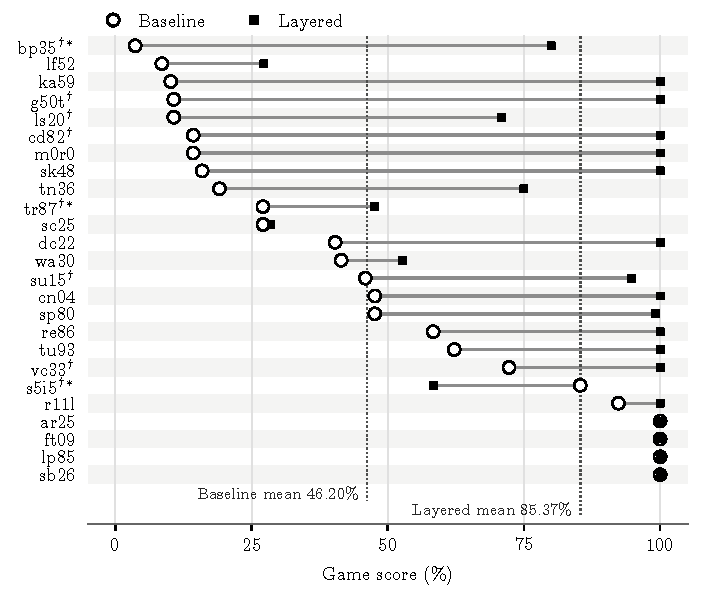
\includegraphics[width=0.66\linewidth]{figures/per_game_scores.pdf}
\caption{\textbf{The layered run scored higher than the baseline run in 20 of 25 games, the same in four, and lower in one.} Each row compares one baseline run and one layered run on the same game, under the same action cap. The rows run from the lowest baseline score to the highest. Open circles show the baseline score, filled squares show the layered score, and a line connects the two. The dotted lines mark the two mean scores. A dagger marks games used or studied during development. An asterisk marks layered runs stopped by repeated timeouts; the figure reports their scores at the point they stopped. The connecting lines show differences between two recorded runs; they do not show statistical uncertainty. Figure~\ref{fig:per-game-outcomes} adds levels completed and actions used.}\label{fig:per-game-scores}
\end{figure}


\Needspace{6\baselineskip}
This paper makes three contributions.
\begin{itemize}
\item \textbf{A layered harness} (Section~\ref{sec:layers}). I added four memory layers to the baseline harness, which had none of them. Figures~\ref{fig:lesson-game-over}--\ref{fig:level-brief} illustrate the layers with examples from the evaluated runs.
\item \textbf{A whole-game comparison on all 25 public games} (Sections~\ref{sec:result-score}--\ref{sec:result-budget}). I ran each harness once per game under the same per-game action caps. The layered harness scored 85.37\% RHAE, compared with 46.20\% for the baseline, completed 166 of 183 levels, compared with 125, and used 35.5\% fewer actions. Replaying the recorded actions through the ARC service confirmed both scores.
\item \textbf{Controlled tests of the level-brief package} (Section~\ref{sec:result-brief}). This package holds the level brief, the rule list, and two supporting features. Under a decision rule fixed before testing, it completed more levels in both test sets and met the benefit criterion in the second.
\end{itemize}

The thesis of this paper is that a language-model agent acts more efficiently on ARC-AGI-3 when its harness keeps the model's own lessons, rules, and notes about the board available at every decision. On these public games, the harness with all four layers performed better than the baseline. Because the whole-game comparison enabled all four layers together, it cannot determine how much each layer contributed. I used or studied eight of the tested games during development, and baseline summaries from all 25 informed it, so the results do not establish performance on unseen games. Section~\ref{sec:discussion} discusses these limits and the replication needed to address them. Appendix~\ref{app:analysis} presents the earlier 100-action baseline analysis and a two-game study of another system as context.

\Needspace{8\baselineskip}
\section{Background and Related Work}\label{sec:background}
Chollet described agent intelligence in terms of how efficiently an agent learns new skills, taking account of its prior knowledge and experience \citep{chollet2019measure}. In ARC-AGI-3, an agent learns through interaction: it explores an unfamiliar game, infers its goal, and determines how different actions affect it \citep{arc2026technical}. ReAct alternates between reasoning about a task and taking actions \citep{yao2023react}, while Reflexion keeps the agent's written reflections on task feedback for use in later trials \citep{shinn2023reflexion}.

Some agents store what they learn about a game in a world model—a program that represents how the game works. Rodionov studied agents that built game simulators, simplified those models, and checked them by replaying recorded actions. The checks required the simulator to reproduce the recorded observations exactly \citep{rodionov2026worldmodels,rodionov2026components}. Tycho chooses actions, examines the results, and can write programs to model the game \citep{lehmann2026tycho}. Kepler tests programs containing proposed game rules by checking whether they predict the changes observed after an action \citep{wu2026kepler}.

Lehmann and Vahdati studied models that built and revised their own harnesses. The models used five development games to guide their revisions. They scored every harness version on twenty separate games whose results never guided those revisions \citep{lehmann2026harness}. I evaluated on 25 public games, eight of which I used or studied during development. My results therefore do not establish performance on unseen games.

Replaying the saved actions through the ARC service checked the recorded observations and scores without generating new model decisions. This check is separate from an independent Verified Leaderboard evaluation \citep{arc2026policy}.

Tycho and Kepler both reported higher scores on the same 25 public games than the 85.37\% reported here. Tycho reported 88.49\% RHAE with Claude Opus 4.8, and 100.00\% with both Claude Opus 5 and GPT-5.6 Sol \citep{lehmann2026tycho}. Kepler reported 100.00\% with Claude Opus 5 \citep{wu2026kepler}. In both systems, the model writes programs that model the game and tests them against its observations. My harness presented the boards and observation summaries as text, together with the model’s earlier hypotheses, lessons, rules, and level brief. The model could not call tools. Because these studies differ in models, tools, and budgets, the scores do not show how much of the score difference comes from any one of those factors. Appendix~\ref{app:followup} presents my earlier two-game Tycho study as historical context.

\section{Methods}\label{sec:methods}
This study is quantitative. It compares two harnesses on the same 25 games by their scores, completed levels, actions, and reported tokens. The examples from the runs show how each memory layer worked; they are illustrations, not measurements.

\subsection{Task, information, and scoring}
\subsubsection{Interaction and information}
I evaluated the baseline and layered harnesses on the same versions of 25 public games, containing 183 levels in total. Before each decision, the model received the current board, the numeric identifiers of the actions currently allowed, the game state, the number of completed levels, and selected earlier observations and action records. The controller executed the action specified in the model's reply and could reset the level after a game over. Each reset counted toward the action cap.


The model could not call tools, retrieve information from external sources, inspect game files, or use memory from other games. Prompts contained no game-specific hints. These restrictions applied to the baseline and layered harnesses evaluated here. The historical Tycho study in Appendix~\ref{app:followup} used different restrictions.


\subsubsection{Primary metric (RHAE)}
The primary metric is Relative Human Action Efficiency (RHAE), which combines level completion with action efficiency relative to a human baseline. Higher scores are better. The benchmark scores each game separately and then averages the game scores, giving each game equal weight \citep{arc2026scoring}.

I use $G$ for the number of games, with $G=25$ for both the baseline and layered harnesses. Game $g\in\{1,\ldots,G\}$ contains $L_g$ levels. For level $\ell\in\{1,\ldots,L_g\}$, I set $d_{g\ell}=1$ if the agent completed the level and $d_{g\ell}=0$ otherwise. I use $a_{g\ell}$ for the agent's action count recorded by the scorer and $b_{g\ell}$ for the official human-baseline action count. The level efficiency is
\begin{equation}
q_{g\ell}=\begin{cases}
\min\{1.15,(b_{g\ell}/a_{g\ell})^2\},&d_{g\ell}=1,\\
0,&d_{g\ell}=0.
\end{cases}\label{eq:level}
\end{equation}
An incomplete level contributes a score of zero. For a completed level, efficiency is the squared ratio of the human-baseline action count to the agent's action count, capped at 1.15.

Within each game, level $\ell$ has weight $\ell$, so later levels count more. The total level weight, $W_g$, and the weighted fraction of levels completed, $C_g$, are
\begin{equation}
W_g=\sum_{\ell=1}^{L_g}\ell=\frac{L_g(L_g+1)}{2},\qquad
C_g=\frac{\sum_{\ell=1}^{L_g}\ell d_{g\ell}}{W_g}.\label{eq:completion}
\end{equation}
The percentage game score, $S_g$, uses the weighted mean efficiency but cannot exceed the \emph{completion cap}, $100C_g$. RHAE is the mean of these game scores.
\begin{equation}
S_g=100\min\left\{C_g,\frac{\sum_{\ell=1}^{L_g}\ell q_{g\ell}}{W_g}\right\},\qquad
\operatorname{RHAE}=\frac{1}{G}\sum_{g=1}^{G}S_g.\label{eq:score}
\end{equation}
Efficiency above 1 cannot raise a game's score above its completion cap. Completing every level does not guarantee a score of 100\%. The agent also has to complete the levels efficiently relative to the human action counts.

I recalculated the final baseline and layered-harness scores using the per-level action counts and human baselines stored with the final replay records. The recalculated scores were 46.19821647\% and 85.36898706\%, respectively, reported as 46.20\% and 85.37\%. Appendix~\ref{app:analysis} retains the historical 100-action scoring analysis.

\subsection{Shared baseline and execution process}\label{sec:harness}
Both the baseline and layered harnesses used Claude Opus 5.5 with high effort through the Claude Code command-line interface (CLI), version 2.1.318. They shared the \texttt{hypotheses} stage of \code{research/claude_arc_v1} as their baseline implementation \citep{dai2026code,dai2026layered}. For each decision, the harness started a new CLI session and sent the prompt together with the required JSON response format. I configured the CLI to disable tools, reuse of saved model sessions, project-specific settings, and external connections. To give the model memory between decisions, the harness included the game's saved observations and notes in later requests. The study did not train or fine-tune the model.


The baseline represented each board as rows of hexadecimal color codes and summarized which cells changed between observations. Each request included the current board, up to two earlier full boards, the eight most recent actions, and up to eight hypotheses written by the model. The harness retained these hypotheses across levels and resets within a game, then cleared them before the next game.

Before executing an action, the harness checked that the action was currently allowed, its coordinates were valid, and the reply followed the required JSON structure. If the model cited an earlier board or action result, the harness checked that the reference used an identifier assigned to that record. These checks enforced the required model reply format and reference rules. They did not establish whether the cited evidence supported the model's claim.

Appendix~\ref{app:prompts} reproduces the instructions given to the model (the system prompt) and the required JSON reply structure used in the original 100-action baseline.

\subsection{Memory layers}\label{sec:layers}
The layered harness added four memory layers to the baseline: lessons from game overs or unchanged boards, an object ledger that grouped board regions and stored the model's notes about them, a separate rule list kept across decisions, and a brief for the new level. The baseline included none of these layers.

Table~\ref{tab:feature-configurations} lists the features behind each layer and which of them each configuration enabled. One distinction matters for the controlled tests. The level brief is one layer. The \emph{level-brief package} is the harness setting \texttt{level\_brief}, which enabled the rule list and the brief together with two supporting features. The following sections explain each feature.

\begin{table}[htbp]
\centering\small
\setlength{\tabcolsep}{5pt}
\begin{tabularx}{\linewidth}{@{}Ycccc@{}}\toprule
 & \multicolumn{2}{c}{Whole-game comparison} & \multicolumn{2}{c}{Level-brief tests}\\
\cmidrule(lr){2-3}\cmidrule(l){4-5}
Feature & Baseline & Layered & \shortstack{Without\\package} & \shortstack{With\\package}\\\midrule
\multicolumn{5}{@{}l}{\emph{Baseline evidence}}\\
\quad Current board, up to two earlier boards, eight recent actions, and up to eight hypotheses & Yes & Yes & Yes & Yes\\\addlinespace[3pt]
\multicolumn{5}{@{}l}{\emph{Layer 1: lessons}}\\
\quad Lessons after game overs & No & Yes & Yes & Yes\\
\quad Lessons after no-effect actions & No & Yes & Yes & Yes\\
\quad Model checked actions against lessons & No & Yes & Yes & Yes\\\addlinespace[3pt]
\multicolumn{5}{@{}l}{\emph{Layer 2: object ledger}}\\
\quad Object ledger, notes, and target checks & No & Yes & Yes & Yes\\\midrule
\multicolumn{5}{@{}l}{\emph{Level-brief package: layers 3 and 4, with two supporting features}}\\
\quad Layer 3: separate persistent rule list & No & Yes & No & Yes\\
\quad Layer 4: brief at level transitions & No & Yes & No & Yes\\
\quad Completion feedback: selected frame and changes & No & Yes & No & Yes\\
\quad Flags for newly observed appearance groups & No & Yes & No & Yes\\\bottomrule
\end{tabularx}
\caption{The table lists the features that each configuration enabled. Yes means enabled, with information supplied when applicable. The whole-game comparison switched on every layer at once. The level-brief tests switched only the level-brief package on and off, in both test sets. All four configurations turned off the optional feature for comparing similar board patterns \citep{dai2026layered,dai2026brieftests}.}\label{tab:feature-configurations}
\end{table}

Figure~\ref{fig:harness} shows how the controller prepared the model's input, checked the reply format and whether the selected action was allowed, and executed an accepted action \citep{dai2026layered}. Figures~\ref{fig:lesson-game-over}--\ref{fig:level-brief} show examples from the evaluated runs. They illustrate how the layers worked, but do not measure each layer's effect on performance.

\begin{figure}[htbp]
\centering
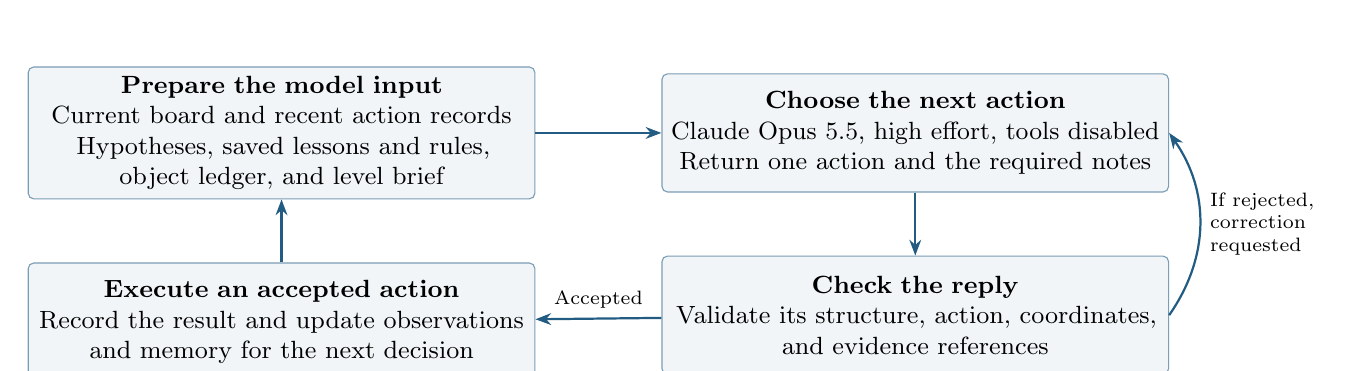
\begin{tikzpicture}[node distance=8mm and 16mm,box/.style={draw=accent!60,fill=wash,rounded corners=2pt,align=center,text width=6.2cm,minimum height=15mm,font=\small},arr/.style={-{Stealth[length=2mm]},draw=accent,thick}]
\node[box] (evidence) {\textbf{Prepare the model input}\\Current board and recent action records\\Hypotheses, saved lessons and rules,\\object ledger, and level brief};
\node[box,right=of evidence] (model) {\textbf{Choose the next action}\\Claude Opus 5.5, high effort, tools disabled\\Return one action and the required notes};
\node[box,below=of model] (check) {\textbf{Check the reply}\\Validate its structure, action, coordinates,\\and evidence references};
\node[box,below=of evidence] (update) {\textbf{Execute an accepted action}\\Record the result and update observations\\and memory for the next decision};
\draw[arr] (evidence)--(model);
\draw[arr] (model)--(check);
\draw[arr] (check)--node[above,font=\scriptsize]{Accepted}(update);
\draw[arr] (update)--(evidence);
\draw[arr] (check.east) to[bend right=35] node[right,font=\scriptsize,align=left]{If rejected,\\correction\\requested} (model.east);
\end{tikzpicture}
\caption{\textbf{The controller prepared evidence, checked the model's reply, and executed the selected action.} The layered harness included all four memory layers in this loop. The baseline used the same execution process with those layers disabled. The controller returned rejected replies for correction before it executed an action. The controller derived records from observed boards and actions, while the model wrote the rules and lessons. Those statements could be wrong. The harness cleared all memory before the next game.}\label{fig:harness}
\end{figure}


\subsubsection{Lessons from failures and unchanged boards}
After a game over, the controller reset the level and the model wrote a lesson about what happened. The harness stored the lesson separately from the baseline's hypothesis list and included it in every later request within the same game. Figure~\ref{fig:lesson-game-over} shows one lesson, from the game over that prompted it to the next request. A lesson recorded the model’s interpretation of its observations. The harness did not verify whether that interpretation was correct.

\begin{figure}[htbp]
\centering\footnotesize
\begin{minipage}[t]{0.42\linewidth}
\setlength{\zoomw}{0.465\linewidth}%
\textbf{1. What the agent observed}\par\vspace{3pt}
\begin{tabular}{@{}c@{\hspace{0.05\linewidth}}c@{}}
\begin{markedboard}[\zoomw]{lessons-game-over-a.png}
\draw[black,line width=0.7pt] (0,0) rectangle (0.25,0.0625);
\end{markedboard} &
\begin{markedboard}[\zoomw]{lessons-game-over-b.png}
\draw[black,line width=0.7pt] (0,0) rectangle (0.25,0.0625);
\end{markedboard}\\[1pt]
Before action 357 & After it: game over\\[5pt]
% the boxed corner of each board, four times larger: 16 cells wide, 4 cells high
\begin{tikzpicture}
\begin{scope}\clip (0,0) rectangle (\zoomw,0.25\zoomw);
\node[anchor=south west,inner sep=0pt] at (0,0) {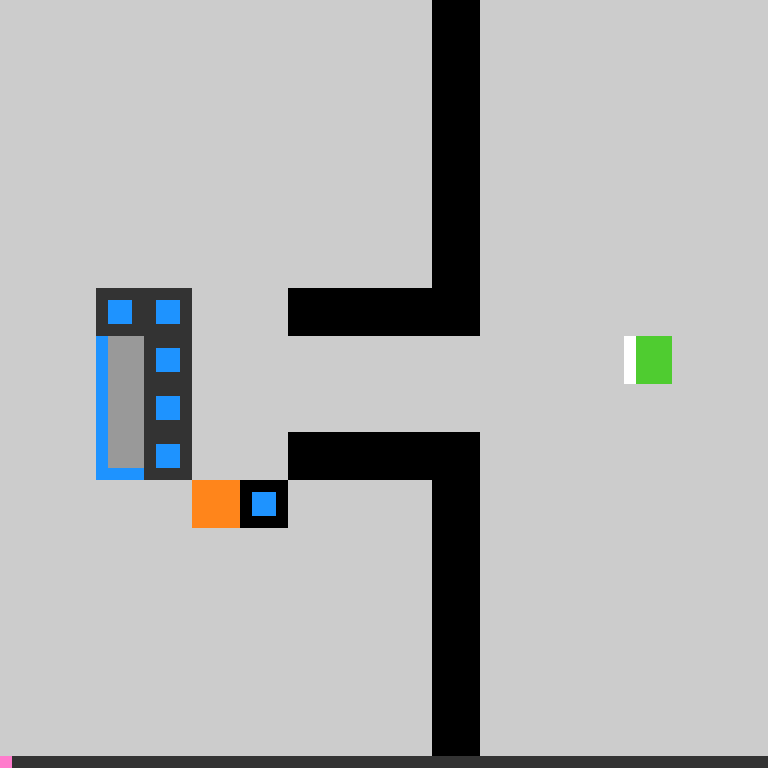
\includegraphics[width=4\zoomw]{figures/runs/lessons-game-over-a.png}};\end{scope}
\draw[black,line width=0.7pt] (0,0) rectangle (\zoomw,0.25\zoomw);
\node[font=\scriptsize,anchor=west,inner sep=1pt] (lab) at (0.2\zoomw,0.16\zoomw) {last pink cell};
\draw[-{Stealth[length=1.6mm]},line width=0.6pt] (lab.west) -- (0.045\zoomw,0.075\zoomw);
\end{tikzpicture} &
\begin{tikzpicture}
\begin{scope}\clip (0,0) rectangle (\zoomw,0.25\zoomw);
\node[anchor=south west,inner sep=0pt] at (0,0) {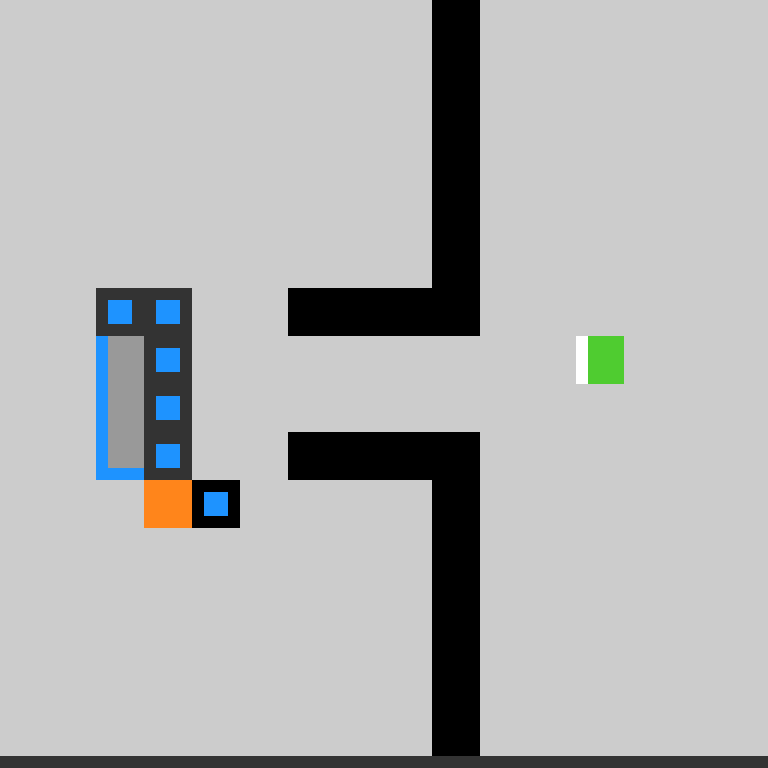
\includegraphics[width=4\zoomw]{figures/runs/lessons-game-over-b.png}};\end{scope}
\draw[black,line width=0.7pt] (0,0) rectangle (\zoomw,0.25\zoomw);
\node[font=\scriptsize,anchor=west,inner sep=1pt] at (0.2\zoomw,0.16\zoomw) {bar empty};
\end{tikzpicture}\\[1pt]
\multicolumn{2}{@{}c@{}}{The boxed corner, four times larger}
\end{tabular}
\end{minipage}\hfill
\begin{minipage}[t]{0.555\linewidth}
\textbf{2. What it stored}, in its reply for action 359\par\vspace{2pt}
\begin{tabularx}{\linewidth}{@{}lY@{}}\toprule
Rule & ``The bar on row 63 is an action budget. Its 7 cells turn to 4 about one every two actions, and the game is over when the last 7 is gone, whatever else is happening on the board.''\\
Applies when & ``Count the 7 cells left on the bottom row and multiply by about 2. If the moves still needed to cover every target tile come to more than that, the attempt will fail. Plan the shortest delivery route from the start and avoid wasted moves.''\\\bottomrule
\end{tabularx}\par\vspace{7pt}
\textbf{3. What the next request showed}, the one for action 360\par\vspace{2pt}
\begin{tabularx}{\linewidth}{@{}lY@{}}\toprule
In the request & The rule and its applies-when clause above, listed under \texttt{game\_over\_lessons} and tagged \texttt{after t357, level 5}\\
The model's check & ``Game-over lesson (budget): 63 of the 64 bottom cells are still 7, so this action will not end the game, and grabbing is needed for the shortest delivery.''\\\bottomrule
\end{tabularx}
\end{minipage}
\caption{\textbf{One game over, the lesson the model wrote from it, and the lesson's return in the next request.} In the layered run of \texttt{wa30}, level 5, action 357 emptied the bar along the bottom row, and the game ended. The controller reset the level, and the model then wrote the lesson in step 2. The harness stored the lesson without checking it and included it in every later request in that game. Step 3 shows the next request and the model's check of its proposed action against the lesson. In the model's text, 7 is the color code of the pink cells and 4 of the dark ones. The model received boards as text; this figure and Figures~\ref{fig:object-ledger} and~\ref{fig:level-brief} draw them in color \citep{dai2026runfigures}. The check in step 3 comes from the run's saved log; the repository records it word for word.}\label{fig:lesson-game-over}
\end{figure}


Some games display a counter or bar that changes as the agent uses actions. The bottom-row bar in Figure~\ref{fig:lesson-game-over} is one, and Figure~\ref{fig:step-counter} in Appendix~\ref{app:no-effect-traces} shows three more. The harness used a heuristic to identify cells belonging to such a counter and excluded them when comparing the boards before and after an action. If no other cells differed, it labeled the action a \emph{no-effect action}. A change in the counter alone therefore did not count as a change to the rest of the board. The class \texttt{CounterMask} in \code{research/claude_arc_v1/recovery.py} of the archived code implements this heuristic \citep{dai2026harnessexport}.

This definition concerns only the compared cells in the final board. Intermediate animation frames could still differ, and game state that was not visible on the board could still change (Figure~\ref{fig:no-effect-examples} in Appendix~\ref{app:no-effect-traces}).

For each no-effect action, the harness kept the action, the board, and a summary of the intermediate frame with the most changed cells relative to the board before the action. The model could write a lesson after taking one additional action and had to write one after taking four additional actions. In later replies, the prompt required the model to check its proposed action against the applicable lessons. These lessons, like those written after game overs, could be wrong.

\Needspace{5\baselineskip}
\subsubsection{Object ledger}
The object ledger recorded detected board regions and the model’s notes about them (Figure~\ref{fig:object-ledger}). The controller identified connected regions, grouped those that looked alike, and recorded where clicks or changes occurred. Each group could contain more than one region on the current board. The model could write notes about a group and select a particular region as the target of its next action. The ledger also marked regions that the agent had not yet clicked and that had not yet changed during recorded play.

The controller detected and grouped regions using fixed rules, which could combine separate objects into a single region or fail to detect relevant objects. The ledger used no object labels or source code provided by the game.

\begin{figure}[htbp]
\centering
\begin{minipage}[c]{0.36\linewidth}
\centering
\begin{markedboard}[\linewidth]{object-ledger-a.png}
\node[note,anchor=west] (aim) at (0.80,0.535) {target on\\this turn};
\draw[pointer] (aim.west) -- (0.762,0.535);
\end{markedboard}
\end{minipage}\hfill
\begin{minipage}[c]{0.60\linewidth}
\footnotesize
\begin{tabularx}{\linewidth}{@{}lrY@{}}\toprule
\shortstack[l]{Appearance\\group} & \shortstack[r]{Detected\\regions} & Model-written note about the group\\\midrule
A & 6 & ``A box. When the player is next to it and facing it, its border turns 3. Action 5 grabs it (border 0). After that, moving toward it pushes it one tile per move. The player can't walk into a box it hasn't grabbed.''\\
AB & 1 & ``An autonomous c block. It moves one tile per player action toward a box, and when it is next to the box it grabs it (the box border turns 4 to 5).''\\
C & 1 & No note yet\\
CY & 1 & No note yet\\
D & 1 & No note yet\\\bottomrule
\end{tabularx}
\end{minipage}
\caption{\textbf{The object ledger grouped regions that looked alike and kept the model's notes about each group across levels.} This example shows \texttt{wa30} at the first decision in level 5, before action 233. Outlines and letters mark the detected regions, and regions with the same letter belong to one appearance group. The table lists the five groups, how many regions each contains, and the notes the model wrote during earlier levels. The arrow marks the region the model chose as its target on this turn: ``I'm aiming at box A at (44,28), the nearest box and right beside the corridor.'' This figure adds the outlines, letters, and arrow; the model received the ledger as text. In the notes, numbers and the letter c are color codes \citep{dai2026runfigures}.}\label{fig:object-ledger}
\end{figure}


\subsubsection{Persistent rules}
The harness kept rules written by the model in a list separate from the baseline's hypotheses and carried the list across decisions within the same game. It held up to 12 rules, each limited to 300 characters. For each rule, the harness stored the level and observation at which it was recorded. When the model replaced a rule, the harness updated the entry with the new rule and its recording information. Once the list was full, the model had to identify an existing rule to replace before adding a new one.

The prompt asked the model to state only what its observations supported and to use less definite wording when the evidence did not support a stronger claim. The harness checked the list size and the identifiers of rules selected for replacement. It did not verify whether the rules were correct.

\subsubsection{Level-transition brief and completion feedback}
Starting with level 2, the model wrote a brief when it entered each level, describing how the previous level ended, what had changed, and what to try next (Figure~\ref{fig:level-brief}).

The brief had four fields. \texttt{won\_by} described how the previous level ended. \texttt{different} described changes in the new level. \texttt{why} gave possible reasons for those changes. \texttt{first} specified the first action to investigate the new level. The harness included the brief in requests throughout the level and allowed the model to correct it.

When the game reported that an action had completed a level, the controller selected an image from that action's animation to help the model understand how the level ended. It excluded the final image, then selected the last remaining image whose dimensions matched the board before the action.

In the next request, the harness showed the selected frame and summarized how its cells differed from the board before the action that completed the level. I call these two items \emph{completion feedback}. If no earlier frame had the required dimensions, the harness reported that it had found no matching frame. Because the selection checked only frame dimensions, the selected frame could already show the next level.

When the object ledger was enabled, the harness flagged groups of board regions whose appearance was not recorded in earlier levels of the same game. A new color or shape did not necessarily mean that a region behaved differently.

The controlled tests compared the package enabled with it disabled, while keeping the object ledger and all other harness settings the same. They measured the package’s combined effect and could not isolate the level brief’s contribution.

\begin{figure}[htbp]
\centering
\begin{minipage}[c]{0.47\linewidth}
\centering
\begin{tabular}{@{}c@{\hspace{6pt}}c@{}}
\begin{markedboard}[0.48\linewidth]{level-brief-a.png}
\node[note,anchor=south west] (won) at (0.04,0.74) {player on the\\last target tile};
\draw[pointer] (0.156,0.74) -- (0.156,0.632);
\end{markedboard} &
\begin{markedboard}[0.48\linewidth]{level-brief-b.png}
\node[note,anchor=north west] (new) at (0.04,0.60) {new block,\\color f};
\draw[pointer] (0.281,0.60) -- (0.281,0.682);
\end{markedboard}\\[1pt]
\footnotesize (a) Completion feedback & \footnotesize (b) First board of level 6
\end{tabular}
\end{minipage}\hfill
\begin{minipage}[c]{0.50\linewidth}
\footnotesize
\begin{tabularx}{\linewidth}{@{}lY@{}}\toprule
Field & What the model wrote (shortened)\\\midrule
\texttt{won\_by} & ``Level 5 completed when the player stepped right onto the last uncovered target tile (8,24). [\ldots] So target tiles covered by the player or by c counted, not only those covered by boxes.''\\
\texttt{different} & ``New things: an f 4x4 block at (16,16). [\ldots] There is no c helper. A wall of 5s, 8 wide, at x44-51, with a gap at rows 24-27.''\\
\texttt{why} & ``Without c, the player has to cover the targets with boxes and/or its own body. The f block is the unknown: maybe a box source, a switch, or a stand-in for a helper.''\\
\texttt{first} & ``Move up toward the f block at (16,16), the new thing, and step next to it to see whether it can be grabbed or reacts.''\\\midrule
Rule added & ``A level completes once every 9-bordered target tile is covered by something: a box, the player, or helper c all count [\ldots].''\\\bottomrule
\end{tabularx}
\end{minipage}
\caption{\textbf{At the start of a new level, the model summarized how the previous level ended and decided what to investigate next.} In the layered run of \texttt{wa30}, action 591 completed level 5. Panel (a) shows the frame the harness selected from that action's animation as completion feedback. Panel (b) shows the first board of level 6. The table quotes the brief the model wrote before its first action in level 6, and the rule it added to its rule list in the same reply. I shortened the quoted text: [\ldots] marks cuts within excerpts, and I also omitted some endings. In the model's text, 5, 9, c, and f are color codes. The brief and the rule are the model's interpretation, which the harness did not check \citep{dai2026runfigures}.}\label{fig:level-brief}
\end{figure}


\subsection{Budgets, validation, and continuation}\label{sec:continuation-design}
I fixed the final cap table on November 18, 2026, before the layered runs began. By then, the baseline had already used 8,402 actions under earlier caps. For 23 of the 25 games, I set the final cap by rounding the whole-game human-baseline action count up to a multiple of 50. For example, the human count of 171 for \texttt{cd82} gave a cap of 200, and the count of 1,843 for \texttt{wa30} gave a cap of 1,850.

Two games kept their earlier caps because the baseline had already won them: \texttt{ft09} kept a cap of 100 despite a human count of 208, and \texttt{sb26} kept a cap of 150 despite a human count of 213. The baseline archive stores the final table. The baseline's later continuations used this table, and each layered run used it from its first action. The caps totaled 17,500 actions across all 25 games for each harness. A run could stop before reaching its game's cap \citep{dai2026continuationfinal}.

The official leaderboard instead gives each level a budget of five times its human-baseline action count and stops the agent once it exhausts that budget \citep{arc2026technical}. I did not enforce this per-level budget during the runs. Section~\ref{sec:result-budget} reports scores recalculated from the recorded action sequences using this budget.

The baseline initially allowed the controller to reset levels up to 10 times across each game. For the baseline continuations, I raised this limit to 50, including for \texttt{tu93}, which had stopped after 10 resets. The layered runs allowed 50 resets per game from the start. Each reset counted toward the game's action cap. The prompts did not tell the model about the reset limit \citep{dai2026continuationfinal}.

For each decision, the controller normally allowed 240 seconds per model call and up to two retries after the initial attempt. For the last 43 recorded actions in \texttt{tr87}, it allowed 400 seconds per call and one retry. The agent completed no additional level during those 43 actions.

Subscription usage limits, slow calls, a lost internet connection, and switches between two subscriptions interrupted some runs. The lost connection stopped \texttt{wa30} at action 1,169. An interrupted run resumed from its saved model replies and game observations, after the runner had checked that it could rebuild every earlier model input exactly. Its earlier actions still counted toward the same cap, so the resumed run was part of the original trial (Appendix~\ref{app:continuation}).

Using the same action caps did not mean that the harnesses made the same number of model calls or sent the same amount of text in each call. The memory layers made model inputs longer, and a rejected reply required another call before the harness could execute a game action. Across the 25 layered runs, the harness rejected 461 of 11,111 replies (4.1\%). Each rejected reply tried to add a rule to the full 12-rule list without identifying an existing rule to replace. Separately, 97 calls exceeded the time limit without returning a reply. Appendix~\ref{app:continuation} gives the full accounting \citep{dai2026logcounts,dai2026wholeverify}.

\subsection{Evaluation design and prior exposure}\label{sec:design}
I compared one recorded baseline run and one recorded layered run per game, played on different days. Here, a run included the model's decisions and game actions, including level resets and any later continuations from saved play. Both the baseline and layered harnesses used the same model identifier, per-game action caps, and shared execution code. They differed in the evidence and memory features enabled.

The baseline combined the original November 6 run, which allowed 100 actions per game, with continuations under larger action caps: first under earlier caps, then under the final cap table (Section~\ref{sec:continuation-design}). Each continuation resumed saved play rather than starting the game again. Each larger cap counted the original and additional actions together. These continuations raised its replay score from 23.16\% to 46.20\% (Table~\ref{tab:main}).

Each layered run began at the first action with all evaluated layers enabled. I ran the layered harness in three batches: first the 11 games on which the baseline scored below 40\%, then 11 more, and then the last three (\texttt{dc22}, \texttt{re86}, and \texttt{wa30}). I wrote the public plan for each batch before its runs began \citep{dai2026layered}.

I did not run repeated whole-game trials to measure variation between runs or test the effects of removing individual layers. The comparison therefore describes these recorded runs and does not estimate variation across repeated trials.

\subsubsection{Development exposure}
The eight games I used to design or tune layers, test their behavior, or study replays were \texttt{bp35}, \texttt{cd82}, \texttt{g50t}, \texttt{ls20}, \texttt{tr87}, \texttt{s5i5}, \texttt{su15}, and \texttt{vc33}. I played levels of \texttt{tr87} and \texttt{cd82} myself, and those observations informed the level brief.

The remaining 17 games were not a held-out test set. I had reviewed baseline summaries across all 25 games, including actions used on unfinished levels, game overs, and repeated boards. These summaries informed harness development.

The controlled level-brief tests described in Section~\ref{sec:brief-design} included sixteen of those 17 games, after I had stopped changing the relevant layer code. These tests began at saved positions from baseline play, except for \texttt{tn36}, which began at the first action. They did not include the remaining game, \texttt{ft09}. Both test sets used the same prompt wording. I made no layer-code changes in response to these tests or the whole-game results.

Throughout the paper, \emph{used or studied during development} refers to the eight games listed above. The appendix retains the original baseline's separate exposure categories. Clearing the agent's memory and omitting hints from its prompts did not remove the researcher's prior exposure to the games.

\subsubsection{Operational interventions and stopping}
Each continuation restored the run’s saved observations, model replies, and accumulated notes. I added no human answers or hints. While preparing to replay the recorded actions, I found an apparent observation mismatch in \texttt{lf52} and discovered that the runner looked for game files in an older folder first. As a precaution, I stopped \texttt{wa30} after 17 actions and restarted it with the toolkit’s files. The reported run used those files from the start. The discarded 17 actions were additional execution work excluded from the results.

Later checks showed that the older files differed only in license comments and unused helper functions. The \texttt{lf52} mismatch affected intermediate animation frames, while the final board matched. The restart therefore proved unnecessary. 

After \texttt{wa30} ended, I corrected a comment in the runner script describing the restart. This correction changed only documentation and did not affect the model’s prompts or the evaluated layer code. No game was rerun because of its score or completion outcome \citep{dai2026replaycorrection}.

Three games---\texttt{tr87}, \texttt{bp35}, and \texttt{s5i5}---stopped after repeated model calls exceeded the time limit. I reported their action and completion counts at the point they stopped. Section~\ref{sec:continuation-design} explains the different time limit and retry allowance used for \texttt{tr87}.

\subsubsection{Local play and action replay}
The comparison used local copies of the public game files. The baseline archive also included the original portion played online. To check the results, I replayed the recorded actions through the ARC service in competition mode, without asking the model to make new decisions (Figure~\ref{fig:evaluation-flow}). The resulting scorecards matched the scores calculated locally \citep{dai2026baselinefinalcard,dai2026finalmanifest}. This replay checked the saved actions and scores; it was not another model trial or an independent Verified Leaderboard evaluation.

All 16,560 baseline actions produced observations that matched the saved records. I checked these matches using hashes, which are short values calculated from every returned image---including animation frames---and the game identifier, game state, level counts, and available actions.

The ARC service accepted all 10,686 layered actions. For 10,661 actions, the observation hashes matched the saved records. The remaining 25 actions, all in \texttt{lf52}, produced matching final boards, game states, and completed-level counts, but different intermediate animation frames. I reported these 25 checks separately because the observations did not match in full \citep{dai2026finalmanifest,dai2026replaycorrection}. Every replay reached the last recorded action, including runs that had stopped before winning.

The three layered scorecards showed updates to the same collection of runs, rather than separate trials. The first reported 82.56\%, with \texttt{dc22}, \texttt{re86}, and \texttt{wa30} still in progress. The second reported 84.14\%, with \texttt{wa30} still in progress and a connection error stopping the \texttt{ls20} replay at action 404 of 800. The final scorecard included every recorded action from all 25 games and reported 85.37\% \citep{scorecard2026layers,scorecard2026layerssecond,scorecard2026finalreplay}.

\begin{figure}[htbp]
\centering
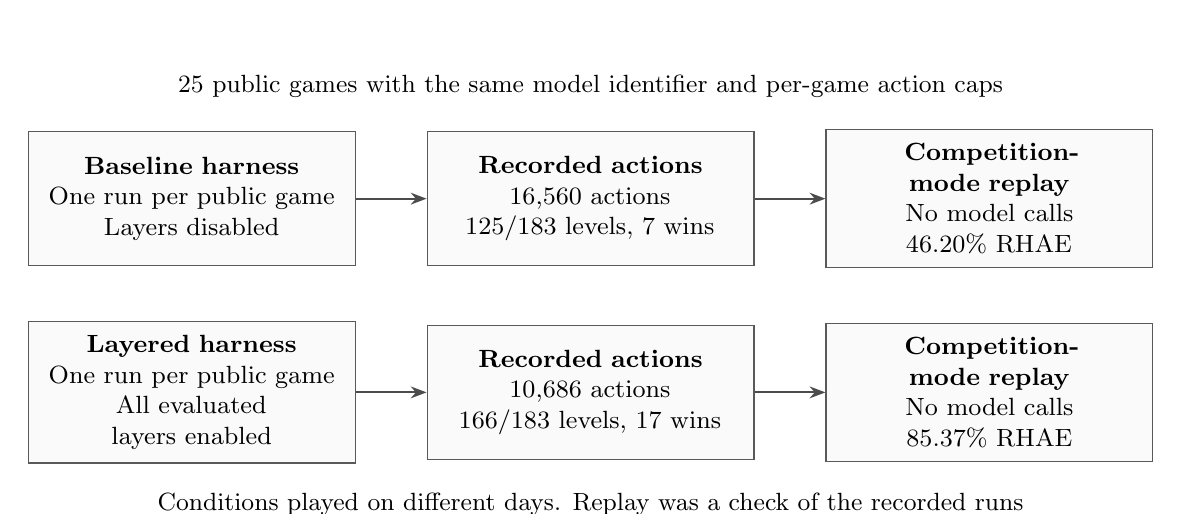
\begin{tikzpicture}[
  node distance=7mm and 9mm,
  run/.style={draw=black!65,fill=black!2,align=center,text width=3.8cm,minimum height=17mm,font=\small,inner sep=5pt},
  arr/.style={-{Stealth[length=2mm]},draw=black!70,thick}]
\node[run] (baseline) {\textbf{Baseline harness}\\One run per public game\\Layers disabled};
\node[run,right=of baseline] (base-record) {\textbf{Recorded actions}\\16,560 actions\\125/183 levels, 7 wins};
\node[run,right=of base-record] (base-replay) {\textbf{Competition-mode replay}\\No model calls\\46.20\% RHAE};
\node[run,below=of baseline] (layered) {\textbf{Layered harness}\\One run per public game\\All evaluated layers enabled};
\node[run,right=of layered] (layer-record) {\textbf{Recorded actions}\\10,686 actions\\166/183 levels, 17 wins};
\node[run,right=of layer-record] (layer-replay) {\textbf{Competition-mode replay}\\No model calls\\85.37\% RHAE};
\draw[arr] (baseline)--(base-record);
\draw[arr] (base-record)--(base-replay);
\draw[arr] (layered)--(layer-record);
\draw[arr] (layer-record)--(layer-replay);
\node[above=3mm of base-record,font=\small,align=center] {25 public games with the same model identifier and per-game action caps};
\node[below=3mm of layer-record,font=\small,align=center] {Conditions played on different days. Replay was a check of the recorded runs};
\end{tikzpicture}
\caption{\textbf{The model first played each game, then I replayed its saved actions to check the recorded results.} During play, the model chose actions using local game files. I then sent the saved actions to the ARC service without asking the model to make new decisions. For every baseline action, the returned observation matched the saved observation in full, including all animation frames. In the layered runs, 10,661 actions matched in full. The remaining 25 actions, all in \texttt{lf52}, matched the final board, game state, and completed-level count, but differed in intermediate animation frames. Replay checked these recorded runs; it did not provide a new model trial or an independent evaluation.}\label{fig:evaluation-flow}
\end{figure}

\FloatBarrier

\subsection{Controlled tests of the level-brief package}\label{sec:brief-design}
I compared two harness configurations that differed only in whether the level-brief package was enabled. Both configurations used lessons written after game overs or actions that had no effect, required the model to check its proposed actions against those lessons, and included the object ledger. I ran each configuration twice on each game, giving four runs per game. Each run allowed up to 100 actions after its starting position and stopped early if the agent won the game. All four runs for a game began at the same saved position from baseline play, except for \texttt{tn36}, where all four began at the first action because its saved baseline run had completed no level.

Before each test, I fixed a decision rule based on levels completed during the new actions. For each game and configuration, I added the completed-level counts from the two runs; levels completed before the starting position did not count. I then compared these per-game counts and their totals across the test set. The package met the benefit criterion, and received the label \emph{helps}, if it completed more levels overall, completed more levels in at least two games, and completed at least as many levels in every game. It received the label \emph{hurts} if it completed fewer levels overall. All other outcomes received the label \emph{no detectable difference}, including mixed outcomes in which the package improved the overall total but performed worse on one game. I applied this rule separately to each test set. These labels describe whether the results met the rule; they are not statistical significance tests and do not establish that the configurations performed equally \citep{dai2026brieftests}.

The seven games in the first test set were \texttt{ar25}, \texttt{ka59}, \texttt{lf52}, \texttt{sc25}, \texttt{sk48}, \texttt{sp80}, and \texttt{wa30}. The nine additional games in the second test set were \texttt{cn04}, \texttt{dc22}, \texttt{lp85}, \texttt{m0r0}, \texttt{r11l}, \texttt{re86}, \texttt{sb26}, \texttt{tn36}, and \texttt{tu93}. The code and prompt wording remained fixed across the two sets.

In the second set, all four runs on each of \texttt{lp85}, \texttt{r11l}, and \texttt{sb26} won the game. Completed-level counts therefore could not distinguish the configurations on those games. I reported the verdict for each test set separately. I disclosed and repeated once any run that ended with an error while calling the model, or whose saved logs failed checks for missing or inconsistent records. The repeat replaced the affected attempt in the verdict, and I interpreted the results only after this procedure. Separate exploratory runs on development games did not contribute to either verdict.

\subsection{Data and resource accounting}\label{sec:analysis-method}
The analysis used the records archived at commit \code{17d00cfdef7944dda9fd9388efa49fccce4877aa} \citep{dai2026harnessexport,dai2026finalmanifest}. This archive contained the final result files from commit \code{5284dc7}, made after all 25 layered runs ended or halted. It also included the log counts reported in Section~\ref{sec:continuation-design}, the figures illustrating the runs, the records behind Figures~\ref{fig:bp35-example}, \ref{fig:lesson-game-over}, and~\ref{fig:step-counter}, and the game-over counts, all of which I added later.

I compared action counts, token usage, and performance, including separate results for games used or studied during development and for the remaining games. These comparisons included one baseline run and one layered run for each of the 25 games. The paper’s supporting files keep earlier scorecards and summaries of unfinished runs as records of results reported before the final evaluation was complete \citep{dai2026baselinefinalcard,dai2026layered,scorecard2026finalreplay,dai2026tokens}.

Reported input usage included uncached input tokens, tokens read from the cache, and tokens written to the cache for later reuse. Reported output usage already included thinking tokens, which the model used for its internal reasoning. I therefore calculated total reported usage by adding input and output once, without adding thinking tokens again.

Calls stopped by the time limit reported no usage, so both the baseline and layered harnesses' token totals excluded them. The layered runs had 97 such calls (Section~\ref{sec:continuation-design}). The reported totals therefore omit an unknown amount of token usage. They do not measure total compute consumed or billing savings.

The final comparison covered all 25 games. It replaced an earlier comparison that excluded \texttt{wa30}, whose layered run was still in progress. I retain the 17.1\% token reduction reported for those 24 games only as a historical result \citep{dai2026tokens}.

\FloatBarrier
\Needspace{24\baselineskip}
\section{Results}\label{sec:results}
The whole-game comparison measured score, level completion, game overs, actions, and token usage on the 25 public games. The controlled tests then examined the level-brief package under the decision rule set in advance. The final subsection reports on the runs that did not win and on earlier tests that found no detectable benefit.

\subsection{The layered runs scored 85.37\% RHAE and the baseline scored 46.20\%}\label{sec:result-score}
Across 25 public games, the layered harness scored 85.37\% RHAE and the baseline scored 46.20\% (Table~\ref{tab:main}). The difference, calculated from the unrounded scores, was 39.17 percentage points. The comparison included one recorded baseline run and one recorded layered run per game, including runs that halted before winning. The layered runs completed 166 of 183 levels and won 17 of 25 games. The baseline completed 125 levels and won seven games. The layered runs used 10,686 actions, compared with 16,560 for the baseline. For example, the layered harness won \texttt{dc22} in 619 actions and \texttt{re86} in 655, while the baseline used its full caps of 1,250 and 1,300 actions on those games and won neither. Both scorecards covered all 25 games \citep{scorecard2026baselinefinal,scorecard2026finalreplay,dai2026baselinefinalcard,dai2026finalmanifest}.

\begin{table}[htbp]
\centering\small
\begin{tabularx}{\linewidth}{@{}Yrrrr@{}}\toprule
Competition-mode replay & RHAE (\%) & Levels & Games won & Actions\\\midrule
\multicolumn{5}{@{}l}{\emph{The comparison: same model and same per-game action caps}}\\
\quad\textbf{Baseline} & \textbf{46.20} & \textbf{125/183} & \textbf{7/25} & \textbf{16,560}\\
\quad\textbf{Layered harness} & \textbf{85.37} & \textbf{166/183} & \textbf{17/25} & \textbf{10,686}\\\midrule
\multicolumn{5}{@{}l}{\color{black!60}\emph{For reference: the same baseline runs after their first 100 actions per game}}\\
\quad\color{black!60}Baseline, first 100 actions & \color{black!60}23.16 & \color{black!60}67/183 & \color{black!60}1/25 & \color{black!60}2,475\\\bottomrule
\end{tabularx}
\caption{The evaluation covered 25 public games, with one recorded run from each harness per game, including halted runs. The two rows in bold are the comparison this paper reports. Both include every recorded action from all 25 ended or halted runs, and the layered runs started from the first action under the extended baseline's cap table. The gray row is not a third condition: it shows the same baseline runs after their first 100 actions per game, before the continuations. ARC-service action replay confirmed all three scores. Resets count as actions. These self-run records do not imply independent leaderboard verification.}\label{tab:main}\label{tab:full-comparison}
\end{table}


Additional actions did not necessarily increase the score. On \texttt{wa30}, the layered harness completed seven of nine levels and used all 1,850 allowed actions. It scored 52.68\%, compared with the baseline's 41.44\%. The agent completed the seventh level at action 1,560. The remaining 290 actions completed no further level, so they used tokens and left the score unchanged.

\subsection{Completion improved in 15 of 25 games and declined in one}\label{sec:result-completion}
The layered harness completed more levels than the baseline in 15 games, the same number in nine, and fewer in one (Figure~\ref{fig:per-game-outcomes}a). It scored higher in 20 games and lower in one (Figure~\ref{fig:per-game-outcomes}b). In the other four games, both harnesses won with scores of 100\%. The only decline in either completion or score occurred on \texttt{s5i5}. The baseline won that game, while the layered run halted after completing six of eight levels. Table~\ref{tab:layered-games} reports each game's final outcome, including runs halted by timeouts.

\begin{figure}[htbp]
\centering
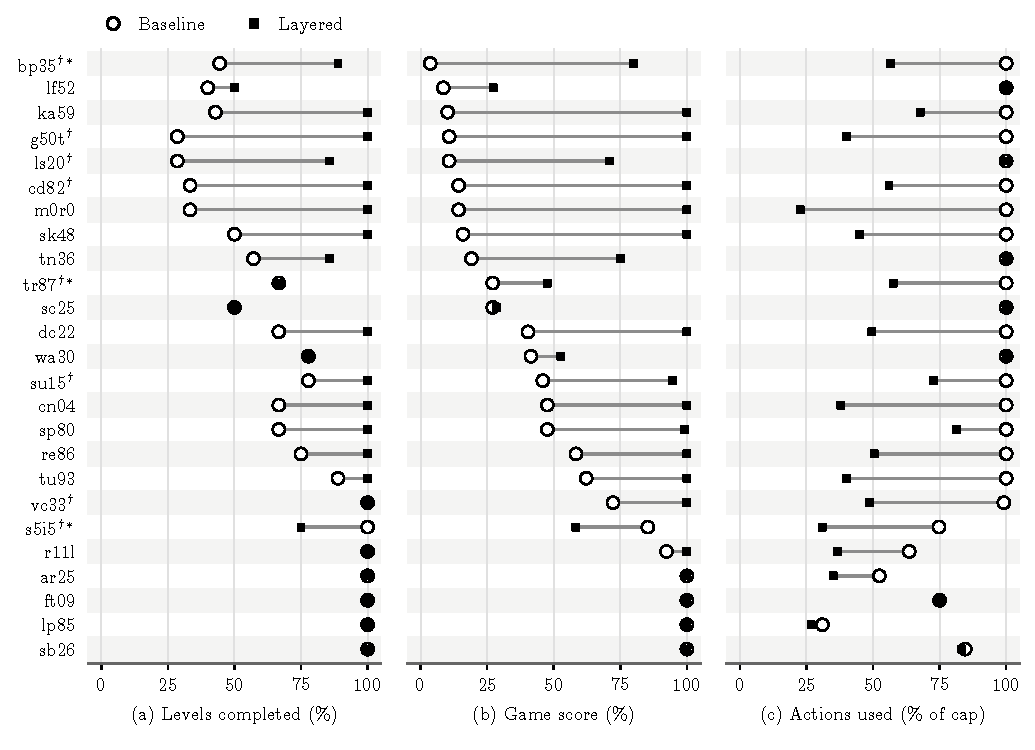
\includegraphics[width=\linewidth]{figures/per_game_outcomes.pdf}
\caption{\textbf{In most games the layered run completed more levels and scored higher while using fewer actions.} Each row compares one baseline run and one layered run on the same game. The rows run from the lowest baseline score to the highest. Open circles show the baseline results, filled squares show the layered results, and a line connects the two. The panels show (a) the percentage of levels completed, (b) the game score, and (c) the percentage of the game's action cap used. Both harnesses had the same cap for each game. A dagger marks games used or studied during development. An asterisk marks layered runs stopped by repeated timeouts; the figure reports their results at the point they stopped. The layered harness completed more levels in 15 games, the same number in nine, and fewer in one (\texttt{s5i5}). It scored higher in 20 games and used fewer actions in 19. The connecting lines show differences between two recorded runs; they do not show statistical uncertainty. Table~\ref{tab:layered-games} gives the exact values.}\label{fig:per-game-outcomes}
\end{figure}

Most of the additional completed levels came from games on which the baseline scored below 40\%. These 11 games formed the first of the three batches of layered runs (Section~\ref{sec:design}). The layered harness completed 66 levels on them, compared with 34 for the baseline, and raised the mean score from 14.69\% to 75.39\%. These 11 games accounted for 32 of the 41 additional levels. On the six games in that set outside the eight-game development group, completion increased from 20 to 35 levels and mean score from 15.86\% to 71.81\%. On the second batch of 11 games, the layered harness completed 79 levels and the baseline completed 74. On the final batch of three games, the layered harness completed 21 levels and the baseline completed 17 \citep{dai2026layered}.

The layered harness had a higher mean score than the baseline in each development-exposure group (Table~\ref{tab:layer-exposure}). On the 17 games outside the eight-game development group, mean score increased from 52.06\% to 87.22\%. On the eight games within that group, it increased from 33.74\% to 81.44\%. Neither group is a held-out test set, because baseline failures on all 25 games informed development (Section~\ref{sec:design}).

\begin{table}[H]
\centering\small
\begin{tabularx}{\linewidth}{@{}Yrrrr@{}}\toprule
Development exposure & Games & \shortstack{Mean score\\baseline / layered} & \shortstack{Levels\\baseline / layered} & \shortstack{Action totals\\baseline / layered}\\\midrule
Other games & 17 & 52.06 / 87.22 & 89 / 113 & 12,178 / 8,048\\
Used or studied & 8 & 33.74 / 81.44 & 36 / 53 & 4,382 / 2,638\\\bottomrule
\end{tabularx}
\caption{The table reports results by development exposure on 25 games, with one run per condition per game, including halted runs. Each pair reports the baseline value followed by the layered value. The eight-game group contains games used to design or tune a layer, or studied during development. Work on \texttt{g50t} consisted of ledger tests and replay study. The other 17 games include \texttt{wa30}. Baseline failures on all 25 games informed development, so neither group is a held-out test set.}\label{tab:layer-exposure}
\end{table}

\subsection{The layered runs had fewer game overs}\label{sec:result-game-overs}
The introduction's example was a repeated game over, so I counted game overs in both sets of runs. The baseline had 127 in 16,560 actions, and the layered runs had 36 in 10,686 actions, or 0.77 and 0.34 per 100 actions. On \texttt{bp35}, the game in that example, the baseline had 22 game overs in 700 actions and the layered run had 5 in 397. These counts include every game over, so they do not show how many repeated an earlier mistake. The baseline count is the number of level resets in its recorded actions: the controller sent one after each game over, and no baseline run ended on a game over \citep{dai2026baselineactions,dai2026layered}.

\subsection{Actions on unfinished levels decreased from 7,940 to 2,170, and reported tokens decreased by 11.0\%}\label{sec:result-resources}
The layered runs used 35.5\% fewer actions overall, 10,686 compared with 16,560. They used fewer actions in 19 games and the same number in six (Figure~\ref{fig:per-game-outcomes}c).

Nearly all of this reduction came from actions used on levels that were unfinished when the runs ended. The baseline used 7,940 actions on its unfinished levels, compared with 2,170 for the layered harness on its unfinished levels. That is a decrease of 5,770 actions, out of an overall decrease of 5,874. The totals for actions used on completed levels were similar, 8,620 for the baseline and 8,516 for the layered harness. Those totals covered different sets of completed levels, with 125 for the baseline and 166 for the layered harness. Relative to the human-baseline action count, the layered harness completed 151 levels at or below that count, compared with 86 for the baseline (Figure~\ref{fig:level-action-ratio}).

\begin{figure}[htbp]
\centering
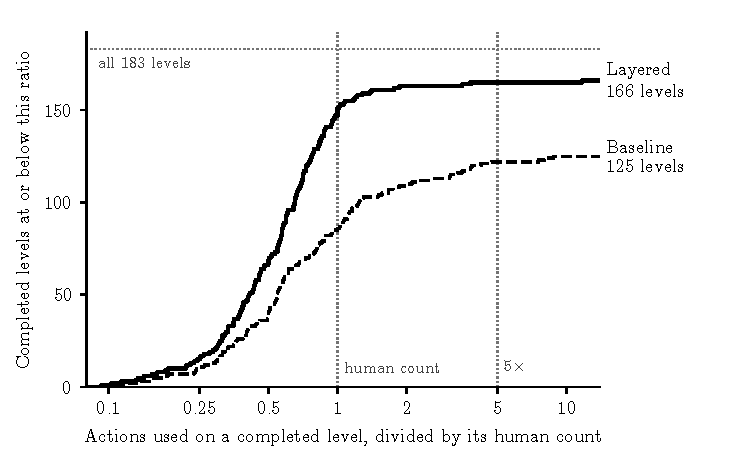
\includegraphics[width=0.74\linewidth]{figures/level_action_ratio.pdf}
\caption{\textbf{Both harnesses solved most of their completed levels within the human action count, and few levels took more than five times that count.} The horizontal axis shows the actions used to complete a level as a multiple of that level's human baseline: 1 means the same number of actions, and 5 means five times as many. The axis uses a logarithmic scale. At each point, a curve shows how many levels a harness completed using no more than that multiple. The solid curve shows the layered runs (166 completed levels), and the dashed curve shows the baseline (125). The vertical dotted lines mark 1 and 5; five times the human count is the official leaderboard's action budget for each level \citep{arc2026technical}. The horizontal dotted line shows the total of 183 levels. The layered harness completed 151 levels within the human action count, compared with 86 for the baseline. One completed level in the layered runs and three in the baseline took more than five times the human count. The curves exclude unfinished levels.}\label{fig:level-action-ratio}
\end{figure}

The overall action totals cover both completed and unfinished games, including runs stopped by timeouts. The three halted runs left 943 actions unused under their caps. On the other 22 games, the layered runs used 34.1\% fewer actions than the baseline, 9,829 compared with 14,924. If the three halted runs had used every remaining action, the overall reduction would have been 29.8\% rather than 35.5\%.

On the six games that both harnesses won, the baseline used 1,324 actions and the layered harness used 881, a reduction of 33.5\%. This subset does not represent performance across all 25 games. It excludes \texttt{s5i5}, which the baseline won and the layered run did not finish before it halted.

\begin{table}[H]
\centering\small
\begin{tabularx}{\linewidth}{@{}Yrrr@{}}\toprule
Reported measure, 25 games & Baseline & Layered & Reduction\\\midrule
Environment actions & 16,560 & 10,686 & 35.5\%\\
\quad on levels left unfinished & 7,940 & 2,170 & 72.7\%\\
\quad on completed levels & 8,620 & 8,516 & 1.2\%\\
Model replies with reported token counts & 16,433 & 11,111 & 32.4\%\\
Input tokens (millions) & 219.307 & 201.030 & 8.3\%\\
Output tokens (millions) & 37.194 & 27.316 & 26.6\%\\
Input plus output (millions) & 256.501 & 228.346 & 11.0\%\\\bottomrule
\end{tabularx}
\caption{The table reports usage for each condition across 25 games, including halted runs and \texttt{wa30}. Reduction is relative to the baseline. The two indented rows split the actions by whether the agent completed the level; the completed levels differ between the harnesses (125 and 166). Reply and token totals include rejected replies retained in the final records; Appendix~\ref{app:continuation} describes the exclusions. Output already includes thinking tokens. Calls stopped by timeouts reported no usage, so the totals for both harnesses exclude them. The layered runs had 97 such calls (Section~\ref{sec:continuation-design}). The totals do not measure total compute consumed or billing savings.}\label{tab:tokens}
\end{table}

Reported token usage decreased by 11.0\%, compared with the 35.5\% reduction in actions (Table~\ref{tab:tokens}). The layered harness used longer requests, and reported input tokens per environment action were 42.1\% higher with the layers. I calculated this average by dividing total reported input tokens by total executed environment actions. On \texttt{wa30}, both the baseline and layered harnesses used 1,850 actions and completed seven levels, but reported tokens increased from 28.408 million to 39.208 million. Including this game reduced the token saving from the earlier 24-game estimate of 17.1\% to 11.0\% across all 25 games \citep{dai2026tokens}.

Two cautions apply to these totals. Calls stopped by timeouts reported no usage, so the totals do not establish a reduction in total compute consumed. The totals do include the extra model calls that the layered harness needed to correct rejected replies: 4.1\% of its replies tried to add a rule to a full list without naming one to replace, and the harness returned them for correction (Section~\ref{sec:continuation-design}).

\subsection{Applying the leaderboard's per-level budget changed each score by less than 0.3 points}\label{sec:result-budget}
The action budget in this study differed from the official leaderboard's. The leaderboard stops an agent at five times the human-baseline action count on each level, whereas this study limited each game's total actions \citep{arc2026technical}. To see how much this difference mattered, I applied the leaderboard's budget to the saved action sequences. For each game, I stopped the saved action sequence when the agent exhausted a level's budget before completing that level, and I discarded all later actions in that game. Applying this cutoff without new model decisions gave scores of 45.92\% for the baseline and 85.13\% for the layered harness, a difference of 39.20 percentage points when calculated from the unrounded scores.

This cutoff removed one completed layered level, the seventh level of \texttt{wa30}, which took 921 actions against a human count of 79. It removed four completed baseline levels. Three exceeded the budget (Figure~\ref{fig:level-action-ratio}) and one followed a level that exceeded the budget in the same game. The calculation could only remove actions from the saved runs. It cannot show what either agent would have done if a different budget had allowed play beyond the study's whole-game action cap.

\subsection{The level-brief package met its benefit criterion in one of two tests}\label{sec:result-brief}
The configuration with the package completed more levels in both test sets, but only the second set met the benefit criterion set in advance (Table~\ref{tab:brief}, Figure~\ref{fig:brief-tests}). In the first set, the package added seven completed levels overall but completed one fewer level on \texttt{wa30}. It therefore failed the requirement to match or exceed completion in every game and received the rule's label \emph{no detectable difference}. In the second set, it added nine completed levels, improved completion in five games, and reduced it in none, meeting the criterion for \emph{helps} \citep{dai2026brieftests}.

\begin{table}[H]
\centering\small
\begin{tabularx}{\linewidth}{@{}YrrrY@{}}\toprule
Test set & Games & \shortstack{Levels\\without / with} & \shortstack{Games\\ahead / behind} & Verdict under the rule\\\midrule
First set & 7 & 10 / 17 & 4 / 1 & No detectable difference\\
Second set & 9 & 29 / 38 & 5 / 0 & Helps\\\bottomrule
\end{tabularx}
\caption{The controlled tests of the level-brief package used two runs per configuration per game and up to 100 new actions per run, stopping early on a win. Runs began from specified restored positions, except \texttt{tn36}, which started at the first action. The configuration without the package retained the other memory layers and object ledger. Level counts sum the two runs for each configuration and include only levels completed during the new actions. Ahead and behind count games where this sum was higher or lower with the package enabled. Verdicts follow the rule set in advance, applied separately to each set (Section~\ref{sec:brief-design}). They are not statistical significance tests.}\label{tab:brief}
\end{table}

\begin{figure}[htbp]
\centering
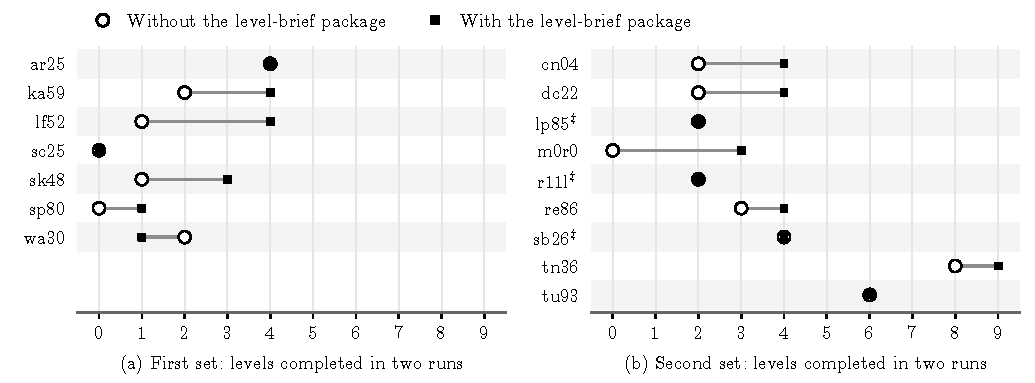
\includegraphics[width=\linewidth]{figures/brief_tests.pdf}
\caption{\textbf{The level-brief package completed more levels in both test sets and completed fewer in one game of the first.} Each row is a game. The horizontal position is the number of levels completed in two runs of up to 100 new actions each. Open circles are the runs without the package, which kept the other memory layers and the object ledger. Filled squares are the runs with it. (a) In the first set, the package was ahead in four games, behind in one (\texttt{wa30}), and level in two, with 17 levels against 10. (b) In the second set, the package was ahead in five games, behind in none, and level in four, with 38 levels against 29. A double dagger marks a game that every run won, so the counts could not differ. Each point sums two runs, and the figure draws no interval.}\label{fig:brief-tests}
\end{figure}


In the second set, every run on \texttt{lp85}, \texttt{r11l}, and \texttt{sb26} won in both tested harness configurations, so the number of completed levels could not distinguish the configurations on those games. These tests do not establish a general benefit or isolate the contributions of persistent rules, completion feedback, the brief, or the flags for newly observed appearance groups. They also did not test the removal of individual layers from whole-game runs.

\subsection{Eight layered runs did not win, and earlier tests gave null or negative results}\label{sec:result-failures}
Eight layered runs did not win. Repeated calls exceeding the time limit halted three of them: after four of six levels on \texttt{tr87}, eight of nine on \texttt{bp35}, and six of eight on \texttt{s5i5}. I retained each run's counts at the point it stopped. The baseline won \texttt{s5i5}, making it the only game in which the layered harness completed fewer levels. The other five runs used their whole action cap: \texttt{wa30} (seven of nine levels), \texttt{ls20} and \texttt{tn36} (six of seven each), \texttt{lf52} (five of ten), and \texttt{sc25} (three of six). Of these five, \texttt{sc25} and \texttt{wa30} ended with the same number of completed levels as the baseline, and \texttt{lf52} with one more.

Four earlier tests during development gave null or negative results. First, stating the scoring rule in the prompt showed no detectable benefit. At 50 saved turns where the baseline had taken an action with no effect, 31 replies chose that action again with the rule in the prompt and 28 without it. Second, I stopped a study of whether the model should reset a level. In its test at ten saved positions, none of 100 replies chose a reset, whether or not the prompt asked the model to consider one. Third, lessons after game overs showed no detectable effect when tested over a whole level. All four runs of \texttt{bp35} level 2, two with the lessons and two without, completed the level. Fourth, an agent with the level brief did not complete \texttt{tr87} level 2 during development \citep{dai2026negatives}. None of these tests showed that the feature it tested helps on its own.

\FloatBarrier
\section{Discussion and Limitations}\label{sec:discussion}
With the same model identifier and action caps, the layered harness completed 41 more of the 183 public-game levels and used 35.5\% fewer actions than the baseline. Most of the reduction was in actions used on levels that each harness left unfinished (Section~\ref{sec:result-resources}), and game overs were less than half as frequent (Section~\ref{sec:result-game-overs}). These results support using the four layers together on the public games tested. If they hold under replication, they indicate that a large part of a language-model agent's score on ARC-AGI-3 depends on what evidence and notes its harness supplies at each decision.

The comparison does not identify which changes accounted for the improvement. All four layers, and the supporting features that accompanied them, changed together. The controlled tests held the other layers fixed while comparing the level-brief package, but that package itself contains four features. Separating their effects would need repeated tests that remove individual layers.

One whole-game run per condition per game does not allow an estimate of variation across repeated runs on the same game. The two harnesses also played on different days, so changes in the model backend over time could have affected the comparison. I did not conduct additional whole-game evaluation trials beyond those reported here, or whole-game tests that removed individual layers.

Equal action caps do not imply equal inference resources. The layers increased input per action, replies rejected for invalid rule-list updates required additional model calls, and calls stopped by timeouts reported no usage. The 11.0\% reduction therefore applies to reported tokens in these runs and does not establish a reduction in total compute consumed.

Prior exposure to the games further limits generalization. Before the final evaluation, I had studied the eight-game development group, inspected baseline failures across all 25 games, played levels of two games myself, and run the controlled level-brief tests with the layer code fixed (Section~\ref{sec:brief-design}). Clearing the agent's memory between games does not remove my own exposure to them. The 17 games outside the development group are therefore not a held-out test set. Differences between the groups could also reflect game difficulty.

Interruptions affected both the completion and the resource comparisons. I retained all three runs halted by timeouts. These halts may have reduced completion, and they shortened the recorded action and token totals. If the halted runs had used every remaining action, the action reduction would have been 29.8\% rather than 35.5\% (Section~\ref{sec:result-resources}).

The checks on the records confirm what the runs recorded, not how the model would act if it ran again. The continuation checks verified that reconstructed requests matched saved requests. Action replay separately checked the recorded actions and scores. For 25 \texttt{lf52} actions, the final board, game state, and completed-level count matched, while intermediate animation frames differed. Neither procedure repeated the model's inference process.

The action budget also differed from the official leaderboard's. Applying the leaderboard's per-level budget to the saved runs changed each score by less than 0.3 points (Section~\ref{sec:result-budget}). That calculation could only remove actions, so it cannot show what either agent would have done under a different budget.

The public records allow readers to reconstruct the scores and reported calculations. The full whole-game requests and replies remain local, so the public repository alone cannot reproduce every audit based on those logs or account for unreported usage.

\subsection{Priority for confirmatory evaluation}
The next priority is a new whole-game comparison that schedules the two harnesses' runs on each game close together and randomizes or balances their order, so that the date of a run cannot explain a difference. The protocol should fix the harness, prompts, game versions, action caps, and inference settings beforehand, together with matched reset, retry, and timeout policies, the number of repetitions, the primary metric, and the analysis. Each run should begin with empty memory. The protocol should also fix the exact model revision where available; otherwise, changes on the provider's side remain a limitation. Repeated paired runs, one from each harness on the same game, would estimate variation across runs on the same game. Where access permits, games that have not informed development would test transfer better than the 17 public games outside the development group. The evaluation record should retain every scheduled run, including halts and failed calls, together with all available usage reports. I have not conducted these confirmatory runs, and the results do not include them.

\section{Conclusion}\label{sec:conclusion}
On 25 public games, with one whole-game run per condition per game, the layered Claude Opus 5.5 harness scored 85.37\% in competition-mode replay, compared with 46.20\% for the baseline. It completed 166 of 183 levels, won 17 games, and used 35.5\% fewer environment actions and 11.0\% fewer reported tokens. Completion improved in 15 games, stayed the same in nine, and declined in one. Under the rule set in advance, one of the two controlled level-brief tests received the label \emph{no detectable difference} and the other the label \emph{helps}. These findings support using the four layers together on the public games. If they hold under replication, they indicate that a large part of a language-model agent's score on ARC-AGI-3 depends on what evidence and notes its harness supplies at each decision. Establishing reliability, individual effects, and transfer needs a new replication with the two harnesses run close together, tests that remove individual layers, and evaluation on previously unused games.

\section*{Reproducibility and Artifact Availability}
The parent project archives the original baseline source at \code{38f41e9d2e9937fd5bcbfbb6fe2c6e126f597039}. The \href{https://github.com/dcw06/ARC-AGI-3-Opus-5.5-Harness/tree/17d00cfdef7944dda9fd9388efa49fccce4877aa}{code and evidence archive}, reviewed at \code{17d00cfdef7944dda9fd9388efa49fccce4877aa}, contains the harness, plans, studies, replay pages, final results, usage report, log counts, game-over counts, and run figures. The plans retain the evaluated files' hashes \citep{dai2026code,dai2026harnessexport}.

The \href{https://arcprize.org/scorecards/0f882c2e-0451-41bd-86c5-211a54785c56}{baseline replay card} and \href{https://arcprize.org/scorecards/96932ddf-ab6a-4354-94b2-9644447dae14}{layered replay card} provide per-game replay and recording links \citep{dai2026baselinefinalcard,dai2026finalmanifest}. I checked public access to both cards and the archived code on November 23, 2026. On November 24, 2026, every link cited or printed in this paper opened without signing in.

The paper's source package is in the \code{paper/} folder of the same repository, on its main branch. It includes the LaTeX source, the closing replay records, per-game and overall results, token report, log counts, game-over counts, and four whole-game result summaries. The file \code{data/final_evidence_provenance.json} lists the source hashes. The command \texttt{python3 verify\_layered.py} reconstructs scores, completion counts, subgroup comparisons, replay acceptance counts, resource reductions, and the per-level budget calculation without model or network calls. The command \texttt{python3 figures/make\_result\_figures.py} redraws Figures~\ref{fig:per-game-scores}, \ref{fig:per-game-outcomes}, \ref{fig:level-action-ratio}, and~\ref{fig:brief-tests} from the same data. These checks do not rerun model inference or measure unreported usage. Earlier interim records and the baseline and Tycho appendices retain their historical scope.

\medskip
\noindent\textbf{AI assistance.} I used Claude Code to develop the harness and experiment tooling, and AI assistance to revise the manuscript and check calculations. The evaluated model and Claude Code are Anthropic products.

\FloatBarrier
\clearpage
\section*{References}
\begingroup
\renewcommand{\section}[2]{}%
\small\raggedright\interlinepenalty=10000
\bibliographystyle{plainnat}\bibliography{references}
\endgroup
\FloatBarrier
\clearpage
\appendix
\section{Layered Per-Game Results and Evidence Status}\label{app:layered}
Table~\ref{tab:layered-games} compares the final baseline and layered runs, using results from their closing scorecards. All 25 layered runs had ended or halted. The End column describes the layered run. W denotes a win, C an action-cap ending, and H a timeout halt. These were local stopping reasons. A replay state of \texttt{NOT\_FINISHED} could still describe a run that reached its action cap.

A dagger marks a game used to design or tune a layer, or studied during development. This includes \texttt{g50t}, which I used for ledger tests and replay study, although I designed no layer on it. The games without a dagger were not a held-out test set.
\begin{longtable}{@{}lrrr rrr c@{}}
\caption{The table gives the final baseline and layered results, which competition-mode replay confirmed. Levels are completed levels divided by available levels. Actions include resets. Scores are RHAE percentages. In the All games row, levels and actions are totals, and scores are equal-game means. End describes the layered run, with W denoting a win, C an action-cap ending, and H a timeout. A dagger marks development exposure, as described above.}\label{tab:layered-games}\\
\toprule
Game & \multicolumn{3}{c}{Baseline} & \multicolumn{3}{c}{Final layered runs} & End\\
 & Levels & Actions & Score & Levels & Actions & Score & \\\midrule
\endfirsthead
\toprule Game & \multicolumn{3}{c}{Baseline} & \multicolumn{3}{c}{Final layered runs} & End\\
 & Levels & Actions & Score & Levels & Actions & Score & \\\midrule
\endhead
\texttt{ar25} & 8/8 & 393 & 100.00 & 8/8 & 263 & 100.00 & W\\
\texttt{bp35}$^{\dagger}$ & 4/9 & 700 & 3.63 & 8/9 & 397 & 80.00 & H\\
\texttt{cd82}$^{\dagger}$ & 2/6 & 200 & 14.29 & 6/6 & 112 & 100.00 & W\\
\texttt{cn04} & 4/6 & 800 & 47.62 & 6/6 & 303 & 100.00 & W\\
\texttt{dc22} & 4/6 & 1,250 & 40.34 & 6/6 & 619 & 100.00 & W\\
\texttt{ft09} & 6/6 & 75 & 100.00 & 6/6 & 75 & 100.00 & W\\
\texttt{g50t}$^{\dagger}$ & 2/7 & 900 & 10.71 & 7/7 & 359 & 100.00 & W\\
\texttt{ka59} & 3/7 & 750 & 10.16 & 7/7 & 508 & 100.00 & W\\
\texttt{lf52} & 4/10 & 1,350 & 8.54 & 5/10 & 1,350 & 27.27 & C\\
\texttt{lp85} & 8/8 & 124 & 100.00 & 8/8 & 107 & 100.00 & W\\
\texttt{ls20}$^{\dagger}$ & 2/7 & 800 & 10.71 & 6/7 & 800 & 70.85 & C\\
\texttt{m0r0} & 2/6 & 1,150 & 14.29 & 6/6 & 260 & 100.00 & W\\
\texttt{r11l} & 6/6 & 159 & 92.35 & 6/6 & 92 & 100.00 & W\\
\texttt{re86} & 6/8 & 1,300 & 58.33 & 8/8 & 655 & 100.00 & W\\
\texttt{s5i5}$^{\dagger}$ & 8/8 & 486 & 85.34 & 6/8 & 201 & 58.33 & H\\
\texttt{sb26} & 8/8 & 127 & 100.00 & 8/8 & 125 & 100.00 & W\\
\texttt{sc25} & 3/6 & 350 & 27.11 & 3/6 & 350 & 28.57 & C\\
\texttt{sk48} & 4/8 & 1,100 & 15.93 & 8/8 & 494 & 100.00 & W\\
\texttt{sp80} & 4/6 & 550 & 47.62 & 6/6 & 447 & 99.17 & W\\
\texttt{su15}$^{\dagger}$ & 7/9 & 400 & 45.89 & 9/9 & 291 & 94.73 & W\\
\texttt{tn36} & 4/7 & 350 & 19.11 & 6/7 & 350 & 75.00 & C\\
\texttt{tr87}$^{\dagger}$ & 4/6 & 450 & 27.09 & 4/6 & 259 & 47.62 & H\\
\texttt{tu93} & 8/9 & 500 & 62.20 & 9/9 & 200 & 100.00 & W\\
\texttt{vc33}$^{\dagger}$ & 7/7 & 446 & 72.27 & 7/7 & 219 & 100.00 & W\\
\texttt{wa30} & 7/9 & 1,850 & 41.44 & 7/9 & 1,850 & 52.68 & C\\
\midrule
All games & 125/183 & 16,560 & 46.20 & 166/183 & 10,686 & 85.37 & \\
\bottomrule
\end{longtable}

The layered runs finished with 17 wins, five action-cap endings, and three timeout halts. They completed 166 levels in 10,686 actions, compared with 125 levels in 16,560 actions for the baseline.

In the layered \texttt{wa30} run, the agent completed level 7 at action 1,560 and reached the cap at action 1,850 without completing level 8. The final manifest recorded its 52.67853748\% game score and all per-level action counts. I stopped an initial attempt after 17 actions as a precaution and restarted the game. Those 17 actions were additional execution work excluded from the reported run. I retained earlier partial cutoffs as historical records.

\textbf{Layered configuration record.} The evaluated layered runs disabled the optional \texttt{pattern\_relations} setting.

\section{Historical Baseline Prompts, Inputs, and Configuration}\label{app:prompts}
This appendix documents the original November 6 baseline, which used a 100-action cap per game. Its prompts, configuration, and exposure ledger were historical records. They did not describe the layered prompts or the eight-game development-exposure grouping used in the main study.

\subsection{Exact system prompt}
The original baseline system prompt concatenated \texttt{SYSTEM}, \texttt{HEX\_NOTE}, and \texttt{RESET\_NOTE} from the archived policy. The text below is exact apart from display wrapping. The machine-readable file preserved it as a single string.
\lstinputlisting{data/system_prompt.txt}

\subsection{User request and response contract}
Each user message was compact JSON with the three fields \texttt{evidence}, \texttt{output\_contract}, and \texttt{procedure}. The evidence included the current observation, recent transitions, the number of omitted transitions, and the model's current hypotheses.

Each current observation contained its observation ID, game ID, game state, completed and target level counts, legal actions, reset flag, omitted-frame count, and final board. Each transition recorded its ID, the chosen action, observed changes, cell changes, and resulting observation. The prediction-check field was empty because prospective prediction output was inactive in this baseline.

The following template illustrates the required response structure; the descriptive strings are placeholders for the values the model had to supply.
\begin{lstlisting}
{"action":{"action_id":"one legal integer from 1 to 7",
           "action_data":"x,y for ACTION6; otherwise {}"},
 "hypotheses":[{"id":"short ID","statement":"testable claim",
   "status":"tentative|supported_locally|contradicted",
   "evidence_ids":["supplied transition or observation ID"]}]}
\end{lstlisting}
The first procedure string was exactly \texttt{Keep competing hypotheses; tie each claim to available evidence. An empty list is allowed.} The harness generated the second string by substituting the number of recorded transitions $n$ in its two numeric positions.
\begin{lstlisting}
evidence_ids may cite any transition so far (t1..t<n>) or observed board (o0 is the initial board, oN the board after tN; o<n> is the current board), including ones no longer shown. A status other than tentative needs at least one such ID.
\end{lstlisting}
Here \texttt{<n>} denotes substitution, not literal prompt text. A retry would add a fourth payload field, \code{previous_reply_rejected}, containing up to 500 characters of rejection feedback. No retry occurred in this run.

The full JSON schema was in \code{schemas/response.schema.json}. It limited action IDs to 1--7, coordinates to integers 0--63, and hypotheses to eight entries. Hypothesis IDs had to contain 1--64 characters, and statements had to contain 1--1,000 characters. The policy parser also checked that the action was currently legal, click actions had exactly the required fields, non-click actions had empty data, references were valid, and non-tentative statuses cited evidence.

\subsection{Model and execution manifest}
Table~\ref{tab:manifest} records the source and runtime used for the original baseline. The evaluated configuration, \code{data/evaluated_config.json}, was an unchanged copy of the archived competition configuration. It included settings shared with other backends. The CLI ignored the API-specific thinking field in this run. The archived source recorded the CLI effort argument, output environment variable, and custom prompt.

\begin{table}[H]
\centering\small
\begin{tabularx}{\linewidth}{@{}P{3.0cm}Y@{}}\toprule
Record & Value or binding\\\midrule
Source archive & \code{38f41e9d2e9937fd5bcbfbb6fe2c6e126f597039} (committed November 6 at 20:50 UTC, after evaluation)\\
Evaluated package & \code{research/claude_arc_v1} (custom CLI backend)\\
Configuration & \code{config/claude_arc_v1.opus55_competition.json}\\
CLI / model & 2.1.318 / \code{claude-opus-5-5} on every returned call\\
ARC SDK requirement & \code{arc-agi==0.9.9} (checked at startup)\\
Run interval & November 6, 2026, 05:41--19:37 UTC\\
Source integrity record & Startup SHA-256 hashes of evaluated Python files and configuration, plus backend version and executable hash\\
Artifact scope & Public scorecard and replays, paper data, and scoring script. Full local inference and event archive not included\\\bottomrule
\end{tabularx}
\caption{The table lists the source and runtime records for the November 6, 100-action baseline. The archived source, the run-start hash records, and the full local event archive are distinct artifacts.}\label{tab:manifest}
\end{table}

\subsection{Completed-game action accounting}
The original 100-action baseline won one game, \texttt{ft09}. Table~\ref{tab:ft09} gives its per-level action counts, human baselines, and efficiencies. Because I had already used \texttt{ft09} for a brief trial run, this win did not show performance on an unseen game.
\begin{table}[H]
\centering\small
\begin{tabular}{@{}rrrrr@{}}\toprule
Level & Agent actions & Human baseline & Level efficiency & Cumulative actions\\\midrule
1 & 4 & 43 & 1.15 & 4\\
2 & 7 & 12 & 1.15 & 11\\
3 & 14 & 23 & 1.15 & 25\\
4 & 16 & 28 & 1.15 & 41\\
5 & 21 & 65 & 1.15 & 62\\
6 & 13 & 37 & 1.15 & 75\\\bottomrule
\end{tabular}
\caption{The table gives the per-level records for \texttt{ft09-0d8bbf25} in the original 100-action baseline. The agent completed all six levels in 75 actions, with no reset. Human baselines were action counts. Level efficiencies followed Equation~\eqref{eq:level}.}\label{tab:ft09}
\end{table}

\section{Baseline Run Records and Reproduction}\label{app:records}
The archived launcher for a new evaluation with the original 100-action baseline code was \code{scripts/run_claude_arc_opus55.sh} \texttt{competition} from the parent-project archive at \code{38f41e9d2e9937fd5bcbfbb6fe2c6e126f597039}. The launcher ran \texttt{python -m research.claude\_arc\_v1.cli} with the competition configuration and confirmations for online ARC evaluation, subscription usage, and competition mode.

Execution required the pinned Python environment, an ARC API key, and Claude CLI access authenticated under the intended account. The paper source contained no credentials. A rerun would consume account allowance and create a new online evaluation. Stochastic model output could produce a different result.

The launcher created a new private directory under \code{.cache/claude_arc_runs}. The CLI recorded the source and backend bindings, created a scorecard, evaluated the current game list in order, closed the scorecard, and ran its record auditor. It used the game versions provided at execution time by the ARC service rather than fixing them to the 25 versions in the archived evaluation.

The paper source provides the following command, which reproduces the archived calculations without making a model call. Table~\ref{tab:artifacts} lists the supporting files.
\begin{lstlisting}
python3 analyze_results.py
\end{lstlisting}

\begin{table}[H]
\centering\small
\begin{tabularx}{\linewidth}{@{}P{5.9cm}Y@{}}\toprule
Shared paper artifact & Contents\\\midrule
\code{data/scorecard_snapshot.json} & Transcribed scorecard, 25 games and 183 levels, with public replay links\\
\code{data/per_game_results.csv} & Versioned outcomes, exposure groups, counted actions, resets, and scorecard states\\
\code{data/level_results.csv} & Integer action totals, human baselines, completion flags, and displayed level efficiencies\\
\code{data/run_summary.csv} & Aggregate run accounting, with measurement source stated for each field\\
\code{data/scoring_audit.json} & Recomputed RHAE, weighted completion, and budget counterfactual\\
\code{data/system_prompt.txt} & Exact evaluated system prompt\\
\code{data/evaluated_config.json} & Unchanged competition configuration\\
\code{data/holdout_ledger.yaml} & Existing development and reduced-exposure partition\\\bottomrule
\end{tabularx}
\caption{The table lists the shared artifacts for the original 100-action baseline. The configuration and ledger are source records. The scorecard tables are transcriptions. Inference totals are run-accounting summaries. The paper source does not include the full local event archive.}\label{tab:artifacts}
\end{table}

\FloatBarrier
\section{Historical Baseline and Tycho Analyses}\label{app:analysis}
Sections D.1--D.3 describe the original November 6 baseline with a 100-action cap per game. Section~\ref{app:followup} records selected November 9 Tycho follow-up cases. Section~\ref{app:continued-audit} reports the baseline after continuation used in the main comparison. Keeping these records separate distinguishes the original 23.16\% result from the final 46.20\% baseline score. Neither the original score decomposition nor the Tycho cases isolates a layer's effect in a whole-game experiment. The original D/R exposure labels below also differ from the layer-design categories used in the main study.

\subsection{Score reconstruction and cap analysis}
The scoring script reconstructed the original 100-action baseline score from the 183 pairs of integer action counts and official human baselines in \code{data/level_results.csv}. It assigned zero to uncompleted levels, calculated completed-level efficiencies using Equation~\eqref{eq:level}, applied the level weights and completion cap, and averaged over 25 games. The reconstructed overall score was 23.16434010\%. Every displayed level and game score matched at its printed precision, and 60 completed levels reached the maximum efficiency of 1.15.

To examine the effect of the 100-action cap, I also calculated a counterfactual in which each level took exactly its official human-baseline action count. I defined the cumulative baseline through level $\ell$ as $B_{g\ell}=\sum_{j=1}^{\ell}b_{gj}$. A level counts as completed in this calculation when $B_{g\ell}\leq100$. I set $d^{H}_{g\ell}=1$ in that case and 0 otherwise. Each completed level had efficiency 1, giving the game score
\[
100\sum_\ell \ell d^{H}_{g\ell}/W_g.
\]
The mean across games was 10.73304473\%. This calculation assumed sequential progression, exact baseline action counts, no exploration overhead, and no resets. It described how the cap interacted with scoring. It did not estimate sampled human performance.

Table~\ref{tab:decomposition} separates the effects of aggregation, level weights, and action efficiency on this original result. Pooled completion gave every level equal weight across all games. Equal-game unweighted completion instead divided each game's completed levels by its own level count, then averaged across games. This gave 37.74921\%. Applying the official level-index weights within each game lowered the mean to 23.28225\%. Applying the observed efficiencies and game completion caps gave 23.16434\% RHAE, a further decrease of 0.11791 percentage points. These were arithmetic recalculations of one run.
\begin{table}[htbp]
\centering\small
\begin{tabularx}{\linewidth}{@{}Yrr@{}}\toprule
Score decomposition & Value (\%) & Change (pp)\\\midrule
Pooled completion $100\sum_g\sum_\ell d_{g\ell}/183$ & 36.61202 & ---\\
Equal-game mean of unweighted completion & 37.74921 & $+1.13718$\\
Equal-game mean of weighted completion & 23.28225 & $-14.46696$\\
RHAE after action efficiency and completion cap & 23.16434 & $-0.11791$\\\bottomrule
\end{tabularx}
\caption{The table decomposes the original 100-action baseline score arithmetically. Each change is the current row minus the preceding row, in percentage points (pp). The changes show the effects of aggregation, level weights, and action efficiency after the game completion cap, respectively. All rows recalculate the same run. I removed and reran no component.}\label{tab:decomposition}
\end{table}


\subsection{Original 100-action game list}
Table~\ref{tab:games} lists all 25 games in the original 100-action evaluation, including the game with zero score. D denotes the original development partition, which included every game with recorded prior exposure. The remaining games were assigned to partitions using a fixed seed and hashes of their full game IDs. R combined the reduced-exposure \texttt{h1} and \texttt{h2} groups from that partition. These labels recorded the original exposure classification; they did not guarantee that R games were unseen, and they differed from the main study's eight-game development group.

In this run, each successful action-selection call produced one model-chosen action, while the controller issued resets. The number of action-selection calls was therefore actions minus resets. The saved scorecard file retains the public replay URLs.
\begin{table}[H]
\centering\small
\setlength{\tabcolsep}{4pt}
\begin{tabularx}{\linewidth}{@{}lcrrrrY@{}}\toprule
Versioned game & Group & RHAE (\%) & Levels & Actions & Resets & Scorecard state\\\midrule
\texttt{ar25-0c556536} & D & 16.67 & 3/8 & 100 & 0 & \texttt{NOT\_FINISHED}\\
\texttt{bp35-0a0ad940} & R & 2.22 & 1/9 & 100 & 3 & \texttt{GAME\_OVER}\\
\texttt{cd82-fb555c5d} & D & 14.29 & 2/6 & 100 & 0 & \texttt{NOT\_FINISHED}\\
\texttt{cn04-2fe56bfb} & R & 14.29 & 2/6 & 100 & 0 & \texttt{NOT\_FINISHED}\\
\texttt{dc22-fdcac232} & R & 4.76 & 1/6 & 100 & 0 & \texttt{NOT\_FINISHED}\\
\texttt{ft09-0d8bbf25} & D & 100.00 & 6/6 & 75 & 0 & \texttt{WIN}\\
\texttt{g50t-5849a774} & D & 3.57 & 1/7 & 100 & 0 & \texttt{NOT\_FINISHED}\\
\texttt{ka59-38d34dbb} & D & 3.11 & 1/7 & 100 & 0 & \texttt{NOT\_FINISHED}\\
\texttt{lf52-271a04aa} & D & 1.82 & 1/10 & 100 & 0 & \texttt{NOT\_FINISHED}\\
\texttt{lp85-305b61c3} & R & 77.78 & 7/8 & 100 & 0 & \texttt{NOT\_FINISHED}\\
\texttt{ls20-9607627b} & D & 10.71 & 2/7 & 100 & 0 & \texttt{NOT\_FINISHED}\\
\texttt{m0r0-492f87ba} & R & 14.29 & 2/6 & 100 & 0 & \texttt{NOT\_FINISHED}\\
\texttt{r11l-495a7899} & R & 71.43 & 5/6 & 100 & 0 & \texttt{NOT\_FINISHED}\\
\texttt{re86-8af5384d} & R & 8.33 & 2/8 & 100 & 0 & \texttt{NOT\_FINISHED}\\
\texttt{s5i5-18d95033} & D & 8.33 & 2/8 & 100 & 0 & \texttt{NOT\_FINISHED}\\
\texttt{sb26-7fbdac44} & R & 58.33 & 6/8 & 100 & 0 & \texttt{NOT\_FINISHED}\\
\texttt{sc25-635fd71a} & D & 27.11 & 3/6 & 100 & 0 & \texttt{GAME\_OVER}\\
\texttt{sk48-d8078629} & D & 8.33 & 2/8 & 100 & 0 & \texttt{NOT\_FINISHED}\\
\texttt{sp80-589a99af} & D & 47.62 & 4/6 & 100 & 1 & \texttt{GAME\_OVER}\\
\texttt{su15-1944f8ab} & D & 6.67 & 2/9 & 100 & 2 & \texttt{GAME\_OVER}\\
\texttt{tn36-ef4dde99} & R & 0.00 & 0/7 & 100 & 1 & \texttt{GAME\_OVER}\\
\texttt{tr87-cd924810} & D & 3.73 & 1/6 & 100 & 0 & \texttt{NOT\_FINISHED}\\
\texttt{tu93-0768757b} & R & 33.33 & 5/9 & 100 & 1 & \texttt{GAME\_OVER}\\
\texttt{vc33-5430563c} & D & 35.71 & 4/7 & 100 & 0 & \texttt{NOT\_FINISHED}\\
\texttt{wa30-ee6fef47} & D & 6.67 & 2/9 & 100 & 0 & \texttt{NOT\_FINISHED}\\
\midrule
All games & & 23.16 & 67/183 & 2,475 & 8 & 1 WIN, 6 GAME\_OVER, 18 NOT\_FINISHED\\\bottomrule
\end{tabularx}
\caption{The table lists all 25 games in the original November 6 baseline, with a 100-action cap per game. It shows scores at scorecard display precision. The final row gives the equal-game mean. Levels are completed levels divided by available levels. D denotes the original development partition. R denotes reduced exposure. Actions include resets. For \texttt{bp35}, \texttt{sp80}, \texttt{su15}, \texttt{tn36}, and \texttt{tu93}, the scorecard showed \texttt{GAME\_OVER}, although the controller reset and continued to the action cap. Only \texttt{sc25} ended in game-over.}\label{tab:games}
\end{table}



\subsection{Platform interaction-tag summaries}
ARC also reported scores by interaction tag. Table~\ref{tab:tags} preserves those platform summaries for the original 100-action baseline. Their aggregation differed from the equal-game RHAE used in the paper.
\begin{table}[H]
\centering\small
\begin{tabular}{@{}lrrrr@{}}\toprule
Platform tag & Tag score (\%) & Levels completed & Actions & Games\\\midrule
\texttt{click} & 24.10 & 21 & 700 & 7\\
\texttt{keyboard} & 6.56 & 6 & 400 & 4\\
\texttt{keyboard\_click} & 19.59 & 34 & 1,300 & 13\\\bottomrule
\end{tabular}
\caption{The table preserves the platform's interaction-tag summaries for the original 100-action baseline. ARC's tag scores are not means of the corresponding game scores, so they are not directly comparable with the equal-game 23.16434\% RHAE. The tag grouping covers 24 games and omits \texttt{ft09}. The full evaluation included all 25.}\label{tab:tags}
\end{table}


\subsection{Follow-up provenance and reference context}\label{app:followup}
I archived the selected Tycho follow-up cases in \code{reports/tycho_opus55_matched_v1} at commit \code{5fd62ecc727963e89c78bf036b97bd03184e4b1f}. The human-readable report was \code{reports/tycho_opus55_matched_v1_results.md}. In the paper source, \code{data/tycho/results.json} preserved the structured outcomes. The files \code{matched_trace.json} and \code{final_trace.json} preserved the action sequences and expected frame hashes. Their replay manifests recorded closed competition-mode cards with no replay failure. These API replays checked deterministic action sequences. They were not new inference trials.

The original 100-action baseline scorecard was \href{https://arcprize.org/scorecards/09cc9d25-ec26-4f26-98f8-9cbd60ec69d7}{\texttt{09cc9d25}} \citep{scorecard2026reported}. The two-game Tycho replay card was \href{https://arcprize.org/scorecards/ac6e3999-e5e4-4488-b981-9d6d80eff73f}{\texttt{ac6e3999}} \citep{scorecard2026tychocard}. For the Tycho \texttt{bp35} continuation, the 427-action checkpoint replay was \href{https://arcprize.org/replay/a8d9ab0a-653c-4e47-8f29-d932551cdd4d}{\texttt{a8d9ab0a}} \citep{scorecard2026bp35checkpoint}, and the completed 474-action replay was \href{https://arcprize.org/replay/b642c1f4-99b6-491f-8e84-813ca4634314}{\texttt{b642c1f4}} \citep{scorecard2026bp35win}. The completed replay's 100\% game score applied to \texttt{bp35} alone.

The three run specifications shared the policy source SHA-256 hash \code{267b1c28f129d4492f1c82a9f503cf3eb5b47c9c836d55e8c8adb3c109eef242}. The recorded overrides first changed \code{TYCHO_MAX_GAME_ACTIONS} from 100 to 0. Here, zero removed the whole-game action cap while retaining the per-level limit of five times the human-baseline action count. They then changed \code{TYCHO_MAX_INFERENCE_COST_PER_GAME} from 100 to 115 US dollars, raising the cumulative inference-cost limit for the game.

The continuation's final manifest reported cumulative usage of 19,450,893 uncached-input, 44,953,313 cache-read, 1,938,558 cache-write, and 558,762 output tokens. Under the archived price schedule,
\[
K=(4N_{\mathrm{uncached}}+0.20N_{\mathrm{read}}+5N_{\mathrm{write}}+20N_{\mathrm{out}})/10^6,
\]
these counts gave a usage cost of \$107.6622646 at the archived API prices. Promotional credits paid for the API usage. Here $K$ is in US dollars. Throughput and builder-activity fields in a resumed manifest could cover only the resumed segment. Accounting for earlier activity therefore required the cumulative result and the complete action record.

For context, ARC Prize published GPT-6 Astra Public Demo sessions using its Provider Adapter harness \citep{arc2026astra}. The archived high-effort \texttt{bp35} session used 488 actions, with per-level counts of 15, 40, 34, 23, 31, 103, 57, 71, and 114 across the nine levels. Across six published effort settings, totals ranged from 430 to 516 actions. Table~\ref{tab:bp35-levels} places the high-effort session beside the Tycho result and official human baselines.

The Astra and Tycho runs differed in model, harness, backend, inference resources, and exposure conditions. Their action counts provided a reference scale. They did not establish superiority or cost efficiency. The archived external session summary, \code{data/tycho/astra_reference.json}, was separate from my experiments.

\begin{table}[H]
\centering\small
\begin{tabular}{@{}lrrrrrrrrrr@{}}\toprule
Level & 1 & 2 & 3 & 4 & 5 & 6 & 7 & 8 & 9 & Total\\\midrule
Official human baseline & 21 & 48 & 44 & 38 & 33 & 87 & 86 & 131 & 163 & 651\\
Tycho + Opus 5.5 & 15 & 49 & 34 & 23 & 35 & 68 & 54 & 57 & 139 & 474\\
Astra, adapter, high & 15 & 40 & 34 & 23 & 31 & 103 & 57 & 71 & 114 & 488\\\bottomrule
\end{tabular}
\caption{The table gives scorer-counted actions by level for \texttt{bp35}. The agent totals include resets. The Astra row is an external reference under different conditions, not a matched model comparison.}\label{tab:bp35-levels}
\end{table}

Running \texttt{python3 verify\_followup.py} reconstructed the follow-up scores and costs, compared the 100-action prefix, checked replay summaries, and checked that the two run-specification changes affected only the recorded budgets. The script made no model or network call. The compressed inference records, model-generated analyses, and the executable world-model artifact remained in the GitHub archive at the cited commit. The model-generated notes and feature attributions were not validated rules or causal evidence.



\subsection{Baseline after continuation and final replay}\label{app:continued-audit}
The baseline used in the main comparison extended the original runs under the archived per-game caps. It completed 125 of 183 levels, won seven games, and used 16,560 actions, including 127 resets. Its third competition-mode replay, card \code{0f882c2e-0451-41bd-86c5-211a54785c56}, confirmed 46.19821647\% RHAE and matched all 16,560 recorded observations \citep{dai2026baselinefinalcard}. Earlier cards recorded intermediate checkpoints. Table~\ref{tab:continued-games} gives the final per-game results.

\begin{table}[H]
\centering\small
\setlength{\tabcolsep}{4pt}
\begin{tabular*}{\linewidth}{@{\extracolsep{\fill}}lrrrrr@{}}\toprule
Versioned game & \shortstack{Replay-confirmed\\RHAE (\%)} & Levels & Actions & Cap & Resets\\\midrule
\texttt{ar25-0c556536} & 100.00 & 8/8 & 393 & 750 & 0\\
\texttt{bp35-0a0ad940} & 3.63 & 4/9 & 700 & 700 & 22\\
\texttt{cd82-fb555c5d} & 14.29 & 2/6 & 200 & 200 & 1\\
\texttt{cn04-2fe56bfb} & 47.62 & 4/6 & 800 & 800 & 4\\
\texttt{dc22-fdcac232} & 40.34 & 4/6 & 1,250 & 1,250 & 4\\
\texttt{ft09-0d8bbf25} & 100.00 & 6/6 & 75 & 100 & 0\\
\texttt{g50t-5849a774} & 10.71 & 2/7 & 900 & 900 & 6\\
\texttt{ka59-38d34dbb} & 10.16 & 3/7 & 750 & 750 & 4\\
\texttt{lf52-271a04aa} & 8.54 & 4/10 & 1,350 & 1,350 & 3\\
\texttt{lp85-305b61c3} & 100.00 & 8/8 & 124 & 400 & 0\\
\texttt{ls20-9607627b} & 10.71 & 2/7 & 800 & 800 & 6\\
\texttt{m0r0-492f87ba} & 14.29 & 2/6 & 1,150 & 1,150 & 7\\
\texttt{r11l-495a7899} & 92.35 & 6/6 & 159 & 250 & 1\\
\texttt{re86-8af5384d} & 58.33 & 6/8 & 1,300 & 1,300 & 3\\
\texttt{s5i5-18d95033} & 85.34 & 8/8 & 486 & 650 & 0\\
\texttt{sb26-7fbdac44} & 100.00 & 8/8 & 127 & 150 & 0\\
\texttt{sc25-635fd71a} & 27.11 & 3/6 & 350 & 350 & 6\\
\texttt{sk48-d8078629} & 15.93 & 4/8 & 1,100 & 1,100 & 3\\
\texttt{sp80-589a99af} & 47.62 & 4/6 & 550 & 550 & 11\\
\texttt{su15-1944f8ab} & 45.89 & 7/9 & 400 & 400 & 7\\
\texttt{tn36-ef4dde99} & 19.11 & 4/7 & 350 & 350 & 2\\
\texttt{tr87-cd924810} & 27.09 & 4/6 & 450 & 450 & 1\\
\texttt{tu93-0768757b} & 62.20 & 8/9 & 500 & 500 & 24\\
\texttt{vc33-5430563c} & 72.27 & 7/7 & 446 & 450 & 2\\
\texttt{wa30-ee6fef47} & 41.44 & 7/9 & 1,850 & 1,850 & 10\\
\midrule
All games & 46.20 & 125/183 & 16,560 & 17,500 & 127\\\bottomrule
\end{tabular*}
\caption{The table gives the final baseline results under the archived per-game action caps, which competition-mode replay confirmed. Levels are completed levels divided by available levels. Actions include resets. The All games row totals the counts and caps and gives the equal-game RHAE of 46.20\%. The baseline won seven games.}\label{tab:continued-games}
\end{table}

For the final baseline \texttt{wa30} run, per-level action counts were $(36,59,187,462,110,70,244,682,0)$, with seven levels completed. The eighth entry counts actions used on the unfinished eighth level; the final zero indicates that level nine was never reached. The corresponding human-baseline counts were $(71,119,183,98,368,68,79,442,415)$. The game score was 41.44187593\%.

Across all games, the baseline after continuation had a mean weighted completion cap of 54.28600289\%. This was the mean of the highest scores permitted by the levels completed in each game, before losses from action inefficiency. Later levels received greater weight, and each game contributed equally to this mean, so it differed from the unweighted completion fraction of 125/183. Its RHAE was 8.08778642 percentage points below that cap after accounting for action efficiency. These calculations described the extended baseline. They did not isolate a policy change.

The original \code{verify_continuation.py} retained its historical checkpoint transcription and offline extension arithmetic. For the final comparison, \code{verify_layered.py} read the final baseline and layered replay records and checked the full 25-game results and reported usage. These arithmetic checks did not launch model runs or independently verify the private restoration logs.


\section{Step Counters and the No-Effect Examples}\label{app:no-effect-traces}
Figure~\ref{fig:step-counter} shows step counters in three games and the cells the harness ignored when it compared boards. Figure~\ref{fig:no-effect-examples} shows two examples from the evaluated runs. Because the harness ignored step-counter cells when comparing final boards, it classified both actions as no-effect actions. The records below give the frame counts and the lessons written by the model.

\begin{figure}[htbp]
\centering
\begin{tabular}{@{}c@{\hspace{8pt}}c@{\hspace{8pt}}c@{}}
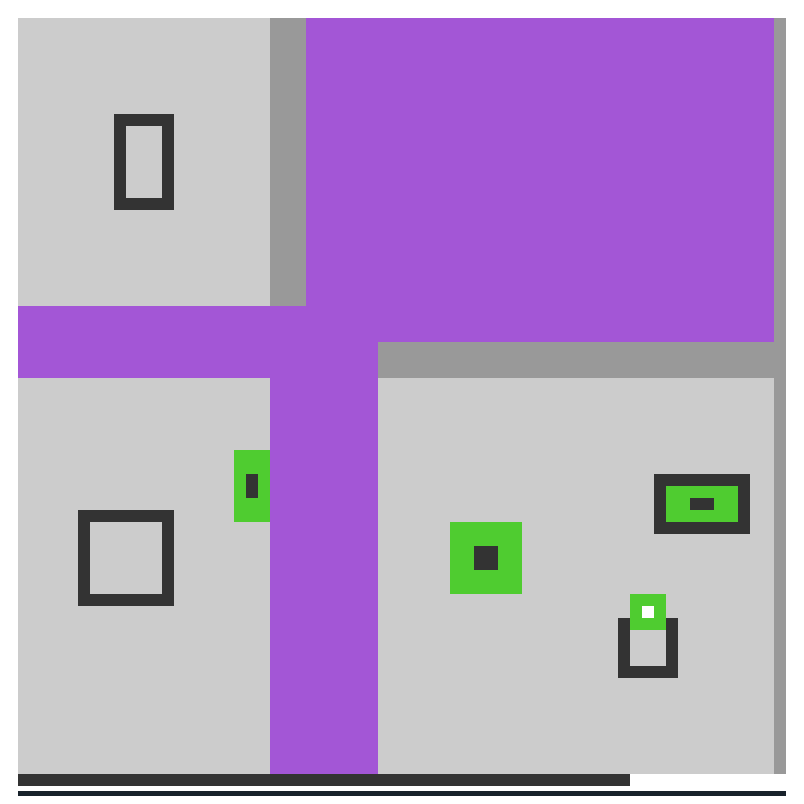
\includegraphics[width=0.29\linewidth]{figures/runs/step-counter-a.png} &
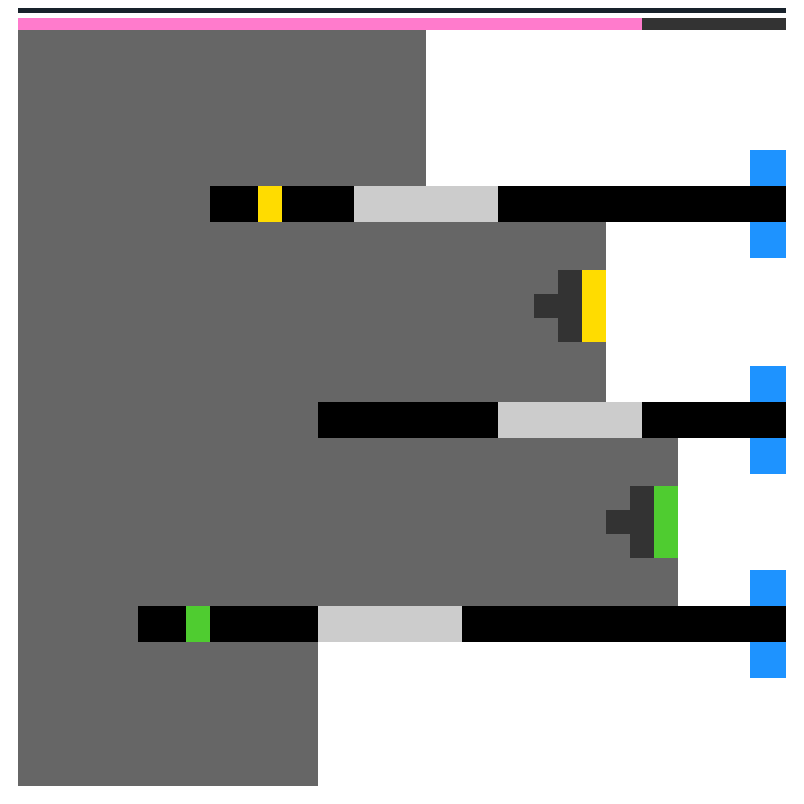
\includegraphics[width=0.29\linewidth]{figures/runs/step-counter-b.png} &
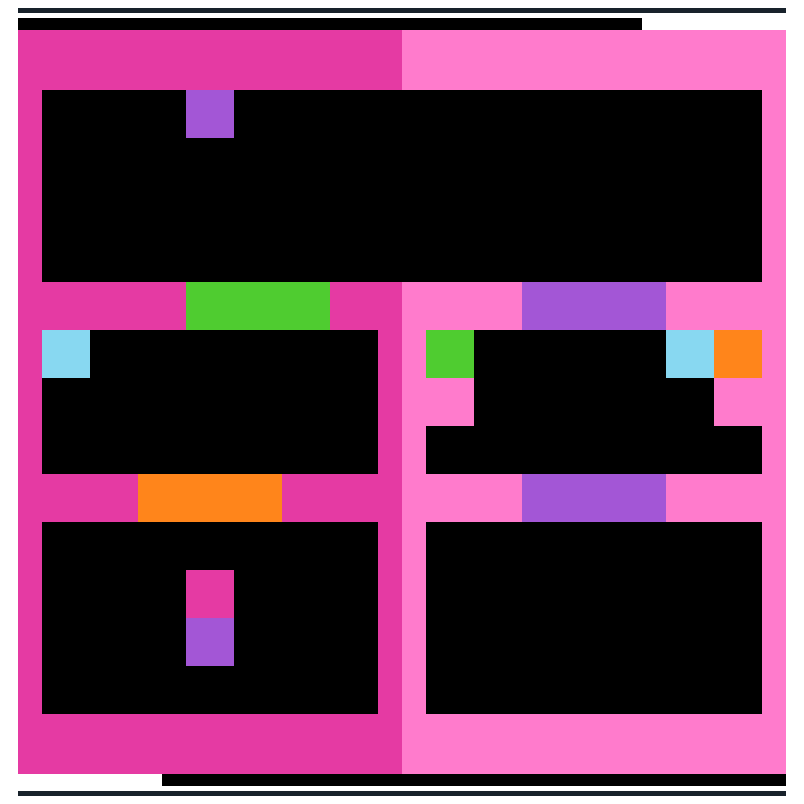
\includegraphics[width=0.29\linewidth]{figures/runs/step-counter-c.png}\\[1pt]
\footnotesize (a) \texttt{ka59}, level 2: bottom row & \footnotesize (b) \texttt{vc33}, level 5: top row & \footnotesize (c) \texttt{m0r0}, level 5: top and bottom rows
\end{tabular}\\[7pt]
\begin{tabular}{@{}r@{\hspace{8pt}}c@{}}
\footnotesize After action 30 & \raisebox{-0.3\height}{\board[0.74\linewidth]{step-counter-d.png}}\\[5pt]
\footnotesize After action 53 & \raisebox{-0.3\height}{\board[0.74\linewidth]{step-counter-e.png}}\\[5pt]
\footnotesize After action 77 & \raisebox{-0.3\height}{\board[0.74\linewidth]{step-counter-f.png}}
\end{tabular}\\[3pt]
{\footnotesize (d) Close-up of the bottom four rows in (a) at three points during level 2}
\caption{\textbf{Some games show a bar that changes as the agent takes actions.} These examples come from the evaluated layered runs. The bar is on the bottom row in (a), the top row in (b), and both the top and bottom rows in (c). The dark lines drawn outside the boards mark the cells the harness ignored when comparing boards. The figure adds these lines. Panel (d) shows a close-up of the bar in (a). Its dark section shrank from 63 cells after action 30 to 51 after action 53 and 39 after action 77. The harness can miss a counter, and some games have no visible counter \citep{dai2026runfigures}.}\label{fig:step-counter}
\end{figure}


\begin{figure}[htbp]
\centering
\begin{tabular}{@{}c@{\hspace{8pt}}c@{}}
\board[0.235\linewidth]{lessons-no-effect-a.png} & \board[0.235\linewidth]{lessons-no-effect-b.png}\\[1pt]
\footnotesize Before action 11, click ringed & \footnotesize After it
\end{tabular}\\[2pt]
{\small (a) \texttt{ka59}, level 1. A click with no final change outside the step counter}\\[8pt]
\begin{tabular}{@{}c@{\hspace{8pt}}c@{\hspace{8pt}}c@{\hspace{8pt}}c@{}}
\board[0.235\linewidth]{frames-between-a.png} & \board[0.235\linewidth]{frames-between-b.png} &
\board[0.235\linewidth]{frames-between-c.png} & \board[0.235\linewidth]{frames-between-d.png}\\[1pt]
\footnotesize Before action 343, click ringed & \footnotesize Frame 5 of 15 & \footnotesize Frame 10 of 15 & \footnotesize Last frame
\end{tabular}\\[2pt]
{\small (b) \texttt{dc22}, level 5. The board changed and changed back}
\caption{\textbf{An action can change the board and then return it to its earlier appearance.} (a) In \texttt{ka59}, level 1, the boards before and after the click differed only in the step counter. (b) In \texttt{dc22}, level 5, the animation changed the board before the final frame returned to its earlier appearance, apart from the counter. The harness classified both actions as no-effect actions because it ignored counter cells in this comparison. Sections~\ref{app:ka59-click} and~\ref{app:dc22-animation} give the frame counts and the model's lessons \citep{dai2026runfigures}.}\label{fig:no-effect-examples}
\end{figure}


\subsection{A click in \texttt{ka59}, level 1}\label{app:ka59-click}
The click at action 11 changed only one bottom-row step-counter cell. After one additional action, the model wrote, ``ACTION6 only does something when it clicks a cell of a 3x3 e-box, which it then selects.''

\subsection{An animation in \texttt{dc22}, level 5}\label{app:dc22-animation}
The click at action 343 returned 15 animation frames. Relative to the board before the click, 38 cells differed in frame 5, 1,575 in frame 10, and 2,830 in frame 14. The final frame differed only in two step-counter cells.

The model received the final board and a summary of the intermediate frame with the most changed cells. From this evidence, it wrote, ``A control that toggles same-colour bridges between solid and checkered will not run while the e marker stands on a bridge that would become checkered. The toggle plays out in the intermediate frames and then reverts, so the final board is unchanged.'' This was the model's interpretation, not a verified game rule. The letter e is a color code \citep{dai2026runfigures}.

\FloatBarrier
\section{Continuation Checks and Call Accounting}\label{app:continuation}
If an interruption stopped a run, the runner used its saved model replies and game observations to restore its progress. Before requesting a new decision, it reconstructed the input shown to the model at each earlier decision and checked that it matched the saved input exactly. It also checked the recorded actions, observations, model name, settings, and action caps. The public experiment plans included a unique identifier, or hash, for each code file to record the exact version used. The resumed run continued from its earlier progress, and its previous actions still counted toward the same cap. It was therefore part of the original trial. I stored the complete logs of model inputs and replies locally and did not include them in the public archive.

Across the 25 layered runs, the harness rejected 461 of 11,111 replies (4.1\%). Each rejected reply tried to add a rule to the full 12-rule list without identifying an existing rule to replace. Five additional replies had the same error, but the model returned them during decisions that an interruption prevented from finishing. When the run continued, the runner started the interrupted decision again. The reported reply and token totals excluded those five replies.

Separately, 97 calls exceeded the time limit without returning a reply. A retry followed 77 of them. The other 20 exhausted the retry allowance and stopped execution. I later resumed some runs from their saved records, so a single run could account for more than one of these stops. Eight other calls failed because a subscription reached its usage limit, and two failed because there was no connection. I counted these events in the local logs using the public script \code{research/level_brief_v1/whole_verify.py} and archived the counts \citep{dai2026logcounts,dai2026wholeverify}.


\end{document}
